\documentclass[11pt]{article}

\usepackage[T1]{fontenc}
\usepackage[utf8]{inputenc}
\usepackage{lmodern}
\usepackage{microtype}
\usepackage[margin=1in]{geometry}
\usepackage{amsmath,amssymb,bm}
\usepackage{booktabs}
\usepackage{tabularx}
\usepackage{multirow}
\usepackage{graphicx}
\usepackage{xcolor}
\usepackage{tikz}
\usetikzlibrary{arrows.meta,positioning,fit}
\usepackage[font=small,labelfont=bf]{caption}
\usepackage{enumitem}
\usepackage{algorithm}
\usepackage{algpseudocode}
\usepackage[hidelinks]{hyperref}
\usepackage[capitalise,noabbrev]{cleveref}

\graphicspath{{figures/}}
\setlength{\emergencystretch}{2em}
\setlist{itemsep=2pt,topsep=4pt}

\newcommand{\Ma}{M_\infty}
\newcommand{\Cp}{C_p}
\newcommand{\CL}{C_L}
\newcommand{\CD}{C_D}
\newcommand{\CM}{C_M}
\newcommand{\vu}{\bm{u}}
\newcommand{\cmd}[1]{\texttt{\small #1}}

\title{A physics-informed neural network and a Fourier neural operator, head to head:\\
\large steady inviscid flow over a family of NACA four-digit airfoils, scored against SU2}
\author{Eder Sousa}
\date{October 2026}

\begin{document}
\maketitle

\begin{abstract}
\noindent
Three learned models are compared with SU2, on steady two-dimensional inviscid compressible flow
around NACA four-digit sections. The models are a Fourier neural operator (FNO), a proper
orthogonal decomposition (POD) baseline and a physics-informed neural network (PINN).
The input space is Mach number $0.30$--$0.80$, angle of attack $-2^\circ$ to $6^\circ$, thickness
$0.08$--$0.16$ and camber $0$--$0.04$, with an extrapolation set at Mach $0.80$--$0.85$.
SU2 ran 1,184 Euler cases on a structured O-grid. The FNO and POD are trained on up to 896 of
them; the PINN is trained on each test case separately, from the equations alone.
Every contestant is scored on the same nodes against SU2 on a $512\times193$ grid, with one force
integrator. Each error is shown beside \emph{the floor}: SU2's own $256\times97$ solution scored
the same way.
In range, the FNO's near-field error is 1.3 times the floor at its $128\times49$ training
resolution and 5.3 times at $256\times97$ on subcritical cases, and 2.4 times on supercritical
cases. In extrapolation every surrogate fails: the FNO is 3.6 times the floor and POD 7.9 times.
The PINN was first built on the Euler equations, and that version converged to fluid at rest. It
was replaced by a full-potential PINN, which is 26--65 times the floor and under-predicts lift
on five of six cases.
On cost, the PINN is 88--220 times SU2 per case, depending on how GPU and CPU time are counted.
The FNO repays its training only after 1,126 new cases.
Three predictions were recorded before any model ran. The first held on wall time only; the
second held; the third held in part.
A fifth stage rebuilt a published transonic Euler PINN with localised artificial
viscosity~\cite{wassing2025} on this study's grid. Under all four tuning configurations it fell
into a uniform stream, and it failed its validation gate at 5.2\,\% Cp error against a 1\,\%
threshold. Nothing probed kept it out of a trivial state: not the slope treatment, the residual
weighting, the optimiser, the embedding, the initialisation, nor hard boundary conditions.
All of this is relative to SU2 at $512\times193$. On the NACA\,0012 anchor, that truth is itself
6--8\,\% below the grid-converged lift of Vassberg and Jameson.
\end{abstract}

\tableofcontents

%===================================================================================================
\section{Introduction}
\label{sec:intro}

The two families of learned flow solvers make opposite bets.
\begin{itemize}
  \item A \emph{neural operator} learns a map from problem parameters to solution fields across a
    whole family of cases~\cite{li2021fno}. It pays a large data and training cost once and then
    answers new cases almost for free.
  \item A \emph{physics-informed neural network}~\cite{raissi2019pinn} needs no data. It is trained
    on one case by minimising the residual of the governing equations at collocation points, and
    it pays the full training cost again for every case.
\end{itemize}
This study measures both bets on one aerodynamic problem, against one truth, with one scorer and a
cost record for every method.

\paragraph{The problem.}
The problem is steady inviscid compressible flow (the Euler equations) around NACA four-digit
sections~\cite{abbott1959}, over a box of four inputs: free-stream Mach number $\Ma$, angle of
attack $\alpha$, thickness $t$ and maximum camber $m$. The range runs from fully subcritical flow
to transonic flow with strong shocks. It is cheap enough that a laptop can generate a thousand
reference solutions with SU2~\cite{economon2016su2}, and hard enough to exercise everything that
makes compressible aerodynamics difficult for learned models:
\begin{itemize}
  \item shocks that move with the inputs;
  \item lift fixed by a condition at a sharp trailing edge;
  \item forces that depend only on the pressure along the wall.
\end{itemize}

\paragraph{The contestants.}
\begin{enumerate}
  \item \textbf{SU2} on the $256\times97$ training grid. This is the reference method, and scored
    against the fine grid it defines \emph{the floor}: the error any $256\times97$ answer carries
    by being on that grid.
  \item \textbf{POD}: a linear basis of training fields, with mode weights interpolated over the
    inputs.
  \item \textbf{FNO}: a Fourier neural operator in the O-grid's index space.
  \item \textbf{PINN}: trained on each test case from the equations, boundary conditions and that
    case's inputs only.
\end{enumerate}
Both networks are written from scratch in PyTorch.

\paragraph{Predictions recorded before any model ran.}
\begin{enumerate}[label=P\arabic*.]
  \item For a single new case, SU2 beats the PINN on cost by one to two orders of magnitude.
  \item The FNO beats ``just run SU2'' only after roughly as many new cases as it took to train it,
    about a thousand, unless the data-efficiency curve shows far fewer training cases suffice.
  \item Without the Kutta condition, the PINN's residuals will look acceptable while its lift is
    wrong.
\end{enumerate}
These are checked in \cref{sec:predictions}.

\paragraph{For readers new to the methods.}
\Cref{app:basics,app:fno,app:pinn,app:compare} explain the learned models in detail, for
teaching. They cover the network building blocks and their training, the FNO as implemented,
the PINN as implemented, and the three models side by side.

\paragraph{How the work ran.}
The comparison ran in five stages (\cref{fig:pipeline}):
\begin{itemize}
  \item S0 checked SU2's accuracy and cost, and froze its settings;
  \item S1 ran the data campaign;
  \item S2 trained the operator models;
  \item S3 ran the PINN;
  \item S4 scored everything.
\end{itemize}
A sixth stage, S5 (\cref{sec:s5}), rebuilt a published Euler PINN with artificial viscosity and
put it through a validation gate. It made predictions of its own.
Every figure quoted here comes from a committed record in \texttt{results/}. The dated log
\texttt{docs/findings.md} gives the command behind each figure.

\begin{figure}[t]
\centering
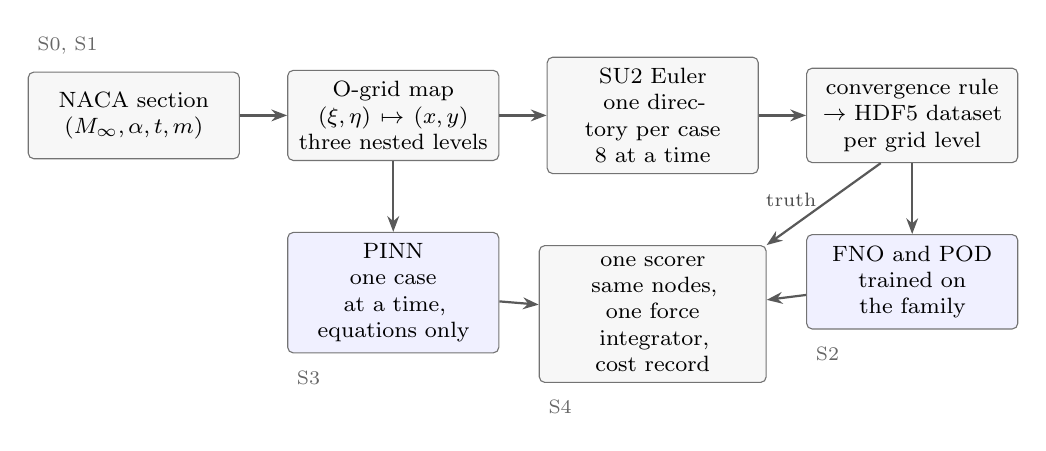
\begin{tikzpicture}[
  node distance=5mm and 6mm,
  box/.style={draw=black!55, rounded corners=2pt, align=center, font=\footnotesize,
              inner sep=4pt, minimum height=11mm, text width=24mm, fill=black!3},
  model/.style={box, fill=blue!6},
  arr/.style={-{Stealth[length=2mm]}, black!65, thick}]
\node[box] (geo) {NACA section\\$(\Ma,\alpha,t,m)$};
\node[box, right=of geo] (grid) {O-grid map\\$(\xi,\eta)\mapsto(x,y)$\\three nested levels};
\node[box, right=of grid] (su2) {SU2 Euler\\one directory per case\\8 at a time};
\node[box, right=of su2] (data) {convergence rule\\$\to$ HDF5 dataset\\per grid level};
\node[model, below=9mm of data] (fno) {FNO and POD\\trained on the family};
\node[model, below=9mm of grid] (pinn) {PINN\\one case at a time,\\equations only};
\node[box, below=9mm of su2, text width=26mm] (score) {one scorer\\same nodes, one force\\integrator, cost record};
\draw[arr] (geo) -- (grid);
\draw[arr] (grid) -- (su2);
\draw[arr] (su2) -- (data);
\draw[arr] (data) -- (fno);
\draw[arr] (grid) -- (pinn);
\draw[arr] (fno) -- (score);
\draw[arr] (pinn) -- (score);
\draw[arr] ([xshift=-4mm]data.south) -- node[font=\scriptsize, black!70, left=1pt, pos=0.45] {truth} (score.north east);
\node[font=\scriptsize, black!60, above=1mm of geo.north west, anchor=south west] {S0, S1};
\node[font=\scriptsize, black!60, below=1mm of pinn.south west, anchor=north west] {S3};
\node[font=\scriptsize, black!60, below=1mm of fno.south west, anchor=north west] {S2};
\node[font=\scriptsize, black!60, below=1mm of score.south west, anchor=north west] {S4};
\end{tikzpicture}
\caption{The pipeline. One function defines the geometry: the mesh generator samples the O-grid map
and the PINN uses it continuously. The models never see the truth, which only the scorer reads.}
\label{fig:pipeline}
\end{figure}

%===================================================================================================
\section{Problem formulation}
\label{sec:problem}

\subsection{Governing equations}

The flow obeys the steady two-dimensional Euler equations in conservation form,
\begin{equation}
  \frac{\partial \bm F}{\partial x} + \frac{\partial \bm G}{\partial y} = 0,\qquad
  \bm F = \begin{pmatrix}\rho u\\ \rho u^2 + p\\ \rho u v\\ \rho u H\end{pmatrix},\quad
  \bm G = \begin{pmatrix}\rho v\\ \rho u v\\ \rho v^2 + p\\ \rho v H\end{pmatrix},
  \label{eq:euler}
\end{equation}
for a perfect gas with $\gamma = 1.4$, where
\begin{equation}
  p = (\gamma-1)\bigl(\rho E - \tfrac12\rho|\vu|^2\bigr),\qquad H = E + p/\rho .
\end{equation}

\paragraph{Boundary conditions.}
On the wall the flow is tangent to the surface, $\vu\cdot\hat{\bm n} = 0$. On a circle of radius
100 chords it meets a uniform free stream at Mach $\Ma$ and angle $\alpha$. SU2 runs dimensionally,
with $p_\infty = 101{,}325$\,Pa, $T_\infty = 288.15$\,K and $R = 287.058$\,J/(kg\,K).

\paragraph{Non-dimensional state.}
Every array a model sees is non-dimensional,
\begin{equation}
  \bm q = (\hat\rho,\ \hat u,\ \hat v,\ \hat p) = (\rho/\rho_\infty,\ u/U_\infty,\ v/U_\infty,\ p/p_\infty).
\end{equation}
The derived quantities used throughout come from one tested module:
\begin{align}
  \Cp &= \frac{\hat p - 1}{\tfrac12\gamma\Ma^2}, &
  M &= \Ma\,\frac{|\hat{\vu}|}{\sqrt{\hat p/\hat\rho}}, \label{eq:cp}\\
  \frac{s - s_\infty}{c_v} &= \ln\frac{\hat p}{\hat\rho^{\,\gamma}}, &
  \frac{H}{H_\infty} &= \frac{\hat p/\bigl(\hat\rho(\gamma-1)\Ma^2\bigr) + \tfrac12|\hat{\vu}|^2}
                            {1/\bigl((\gamma-1)\Ma^2\bigr) + \tfrac12}. \label{eq:entropy}
\end{align}
Two identities make these useful checks:
\begin{itemize}
  \item In shock-free inviscid flow the entropy must stay at its free-stream value, so any rise is
    numerical error.
  \item In steady inviscid flow from a uniform stream the total enthalpy $H$ is constant
    everywhere, through shocks included.
\end{itemize}

\subsection{Geometry}

A NACA four-digit section of unit chord is parameterised as one closed curve of $\xi\in[0,1)$:
$\xi = 0$ is the trailing edge, $\xi\in[0,\tfrac12]$ runs along the lower surface to the leading
edge, and $\xi\in[\tfrac12,1)$ runs back along the upper surface.

\paragraph{Thickness.}
With $s = \cos\pi\xi$, the chord station is $x = s^2$, so $\sqrt{x} = |s|$ and the curve has no
square-root singularity at the leading edge. The signed half-thickness is
\begin{equation}
  y_s(\xi) = -\operatorname{sign}(s)\,5t\left(0.2969\sqrt{x} - 0.1260x - 0.3516x^2 + 0.2843x^3 - 0.1036x^4\right),
  \label{eq:naca}
\end{equation}
where the $x^4$ coefficient closes the trailing edge.

\paragraph{Camber.}
The camber line, with $p = 0.4$ fixed, is
\begin{equation}
  y_c = \begin{cases}\dfrac{m}{p^2}\left(2px - x^2\right), & x < p,\\[2mm]
  \dfrac{m}{(1-p)^2}\left(1 - 2p + 2px - x^2\right), & x \ge p.\end{cases}
\end{equation}
The thickness is applied normal to it: the wall point is
$(x - y_s\sin\theta_c,\; y_c + y_s\cos\theta_c)$, with $\tan\theta_c = \mathrm{d}y_c/\mathrm{d}x$.

The same function runs on NumPy arrays and on PyTorch tensors, so the mesh and the PINN share one
geometry.

\begin{table}[t]
\centering\small
\caption{The input box, the sets and the grids, all fixed before any model was trained.}
\label{tab:box}
\begin{tabular}{@{}lll@{}}
\toprule
\multicolumn{3}{@{}l}{\textbf{Inputs}}\\
Mach number $\Ma$ & $[0.30,\ 0.80]$ & extrapolation set: $[0.80,\ 0.85]$\\
Angle of attack $\alpha$ & $[-2^\circ,\ 6^\circ]$ & \\
Thickness $t$ & $[0.08,\ 0.16]$ & \\
Maximum camber $m$ & $[0,\ 0.04]$ & camber position $p = 0.4$ fixed\\
\midrule
\multicolumn{3}{@{}l}{\textbf{Sets} (scrambled Sobol designs, seeds fixed)}\\
Training & Sobol points 1--896 & $256\times97$\\
Validation & Sobol points 897--1,024 & $256\times97$; tuning and early stopping only\\
Test, in range & 64 points, another seed & $512\times193$ (truth) and $256\times97$ (floor)\\
Test, extrapolation & 16 points, $\Ma\in[0.80,0.85]$ & $512\times193$ and $256\times97$\\
\midrule
\multicolumn{3}{@{}l}{\textbf{Grids} (nested exactly: each level is every second node of the next)}\\
Fine & $512\times193$ & truth\\
Training & $256\times97$ & data, evaluation, the floor\\
Coarse & $128\times49$ & FNO training\\
\bottomrule
\end{tabular}
\end{table}

\subsection{The O-grid}

All data live on one structured O-grid, defined as a continuous map
$(\xi,\eta)\in[0,1)\times[0,1]\mapsto(x,y)$:
\begin{equation}
  \bm x(\xi,\eta) = \bm x_w(\xi) + \sigma(\eta)\,\bigl(\bm x_f(\xi) - \bm x_w(\xi)\bigr),\qquad
  \bm x_f(\xi) = \bigl(\tfrac12 + R\cos(-2\pi\xi),\ R\sin(-2\pi\xi)\bigr),
  \label{eq:ogrid}
\end{equation}
with $R = 100$ chords. The radial distribution is geometric,
\begin{equation}
  \sigma(\eta) = \frac{r^{N\eta} - 1}{r^{N} - 1},\qquad N = 192,
\end{equation}
where the ratio $r$ is chosen so that the first wall spacing of the $256\times97$ grid is
$2\times10^{-3}$ chords.

\paragraph{Nested levels.}
The grids sample the map at $\xi_i = i/N_I$ and $\eta_j = j/(N_J - 1)$. Each coarser level is
therefore exactly every second node of the next, which lets the truth be read at the training
grid's nodes without interpolation. Node $(i,j)$ has SU2 id $jN_I + i$, so every output maps
straight back onto an $(i,j)$ array.

\paragraph{The outer point.}
The outer point sits at the uniform polar angle $-2\pi\xi$. The first construction instead placed
it at the same angle about mid-chord as the wall point. That version folded the mesh: 9,792
inverted cells at $t = 0.08$, $m = 0.04$. The uniform angle has no inverted cell at any corner of
the box (\cref{fig:grid}).

\begin{figure}[t]
\centering
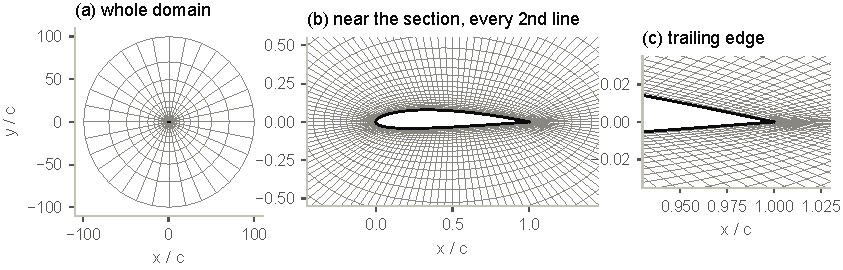
\includegraphics[width=\textwidth]{grid.pdf}
\caption{The $256\times97$ O-grid around a $t = 0.12$, $m = 0.02$ section.
(a) The whole domain, every eighth line around and every fourth outward. (b) Near the section.
(c) The trailing edge, where the section's cosine clustering crowds the lines and makes
$\partial\bm x/\partial\xi$ vanish at the edge itself: $x_\xi = y_\xi = 0$, so the map is
degenerate there ($J = 0$). That point matters for the PINN (\cref{sec:potential}).}
\label{fig:grid}
\end{figure}

%===================================================================================================
\section{Reference data: SU2}
\label{sec:su2}

\subsection{Solver settings and the convergence rule}

\paragraph{Settings.}
SU2 8.5.0 solves \cref{eq:euler} on each case's own mesh, one serial process per case:
\begin{itemize}
  \item a JST scheme~\cite{jameson1981jst} with sensor coefficients $(0.5, 0.02)$;
  \item implicit Euler pseudo-time stepping with an adaptive CFL;
  \item an FGMRES linear solver with ILU preconditioning;
  \item weighted-least-squares gradients.
\end{itemize}

\paragraph{The convergence rule.}
Convergence is judged by a rule of our own, read from the history file, not by SU2's flag. A case
is \emph{converged} if and only if both hold:
\begin{equation}
  \log_{10}\frac{\mathrm{rms}(R_\rho)_{1}}{\mathrm{rms}(R_\rho)_{N}} \ge 5
  \quad\text{and}\quad
  \max_{k\in\mathcal W}C_\bullet^{(k)} - \min_{k\in\mathcal W}C_\bullet^{(k)} \le 10^{-6}
  \ \text{ for } C_\bullet\in\{\CL,\CD\}.
  \label{eq:conv}
\end{equation}
Here $\mathcal W$ is the last 500 iterations. The caps are 10,000 iterations on the training grid
and 20,000 on the fine grid.

\paragraph{Consistency with SU2's own stop.}
SU2 stops when the mean relative change of $\CL$ and $\CD$ over $n_c$ iterations falls below
$\varepsilon_c$. At that stop $\CL$ can still vary by up to $\varepsilon_c n_c|\CL|$ over the
window. The frozen setting therefore has to satisfy
\begin{equation}
  \varepsilon_c\, n_c\, |\CL|_{\max} = 10^{-9}\times500\times1.86 = 9.3\times10^{-7} < 10^{-6},
\end{equation}
where $|\CL|_{\max} = 1.86$ is a thin-airfoil bound at the box's highest-lift corner. Stage S0 found
this the hard way:
\begin{itemize}
  \item with $\varepsilon_c = 10^{-7}$, none of 24 runs met \cref{eq:conv};
  \item with $10^{-8}$, 9 of 23 did;
  \item with $10^{-9}$, all 24 did.
\end{itemize}

\subsection{Stage S0: accuracy and cost}

Five cases were each solved on all three grids:
\begin{itemize}
  \item a symmetric section at $\alpha = 0$;
  \item two subcritical lifting cases;
  \item a supercritical case at $\Ma = 0.75$;
  \item the NACA\,0012 anchor at $\Ma = 0.8$, $\alpha = 1.25^\circ$.
\end{itemize}

\paragraph{Multigrid.}
Three multigrid levels converged every case and agreed on $\CL$ to $3\times10^{-9}$. They cost more
wall time on all five cases (median 239.8\,s against 132.6\,s), so the campaign runs without
multigrid.

\paragraph{Mesh error.}
Writing $f_c$, $f_t$ and $f_f$ for the coarse, training-grid and fine values, the observed order is
\begin{equation}
  \hat p = \log_2\frac{|f_c - f_t|}{|f_t - f_f|}.
\end{equation}
It was negative or non-monotone for $\CL$ on every lifting case. The three grids are therefore not
in the asymptotic range, and the error is reported as the plain difference from the fine grid
(\cref{tab:s0}), not as a Richardson extrapolation.

\paragraph{Outer boundary.}
Moving the outer boundary from 100 to 200 chords changed $\CL$ by $1.3\times10^{-3}$ and
$2.1\times10^{-3}$. The radius was kept at 100 chords, so all methods share that far-field
truncation.

\paragraph{Known answers.}
\begin{itemize}
  \item The symmetric case gives $|\CL| = 2\times10^{-15}$.
  \item Subcritical drag, ideally zero, is $-0.74$ to $+1.23$ counts.
  \item The lift slope is 1.129 times the Prandtl--Glauert thin-airfoil value, above it as a 12\,\%
    thick section should be.
  \item The NACA\,0012 anchor gives $\CL = 0.3260$ at $512\times193$, which is compared with the
    grid-converged reference in \cref{tab:vj}.
\end{itemize}

\paragraph{The anchor against a grid-converged reference.}
Vassberg and Jameson~\cite{vassberg2010} solved this case on aspect-ratio-one O-meshes up to
$4096\times4096$ cells, about 150 chords deep, with three solvers. Their Richardson continuum
estimates are $\CL = 0.3482$--$0.3562$ across the solvers (\cref{tab:vj}). Their section is the
NACA\,0012 equation with its standard $x^4$ coefficient, extended to a sharp trailing edge at
$x = 1.0089$; ours closes the edge at $x = 1$. Our grids give coefficients below that range on every
quantity:
\begin{itemize}
  \item at $512\times193$, $\CL$ is 6--8\,\% low, $\CD$ 12--15 counts low, and $|\CM|$
    17--20\,\% low;
  \item the lift is still rising with refinement, from below, while their FLO82 sequence descends
    to the continuum from above.
\end{itemize}
So the truth used for scoring carries its own discretisation error on transonic lifting flow. On
this case it is about 2.6 times the floor's grid difference in $\CL$. The comparison among
contestants is unaffected, because all of them meet the same truth. Statements such as ``near the
floor'' measure agreement with SU2 at $512\times193$, not with the exact Euler solution. The
differences in section, far field (100 against about 150 chords, and no point-vortex correction
here), grid and scheme are not separated.

\begin{table}[t]
\centering\small
\caption{The NACA\,0012 anchor ($\Ma = 0.8$, $\alpha = 1.25^\circ$): this study's SU2 grids
against the four continuum estimates of Vassberg and Jameson~\cite{vassberg2010} (their
Table~11). $\CM$ is compared in magnitude; both are nose-down.}
\label{tab:vj}
\begin{tabular}{@{}lrrrcc@{}}
\toprule
& \multicolumn{3}{c}{This study, SU2} & \multicolumn{2}{c@{}}{Vassberg \& Jameson continuum}\\
\cmidrule(r){2-4}\cmidrule(l){5-6}
& $128\times49$ & $256\times97$ & $512\times193$ & min & max\\
\midrule
$\CL$ & 0.3118 & 0.3174 & 0.3260 & 0.3482 & 0.3562\\
$\CD$ (counts) & 215.2 & 208.8 & 212.3 & 224.5 & 226.8\\
$|\CM|$ & 0.0278 & 0.0288 & 0.0311 & 0.0374 & 0.0388\\
\bottomrule
\end{tabular}
\end{table}

\paragraph{The scorer check.}
The scorer's own force integrator (\cref{sec:scoring}) reproduced SU2's reported $\CL$, $\CD$ and
$\CM$ on all 24 S0 solutions to $4.9\times10^{-11}$, against the required $10^{-6}$.

\begin{table}[t]
\centering\small
\caption{S0: the training grid minus the fine grid (the floor, on the S0 cases), and the cost per
case. $\CD$ is in counts ($10^{-4}$); $\Cp$ is compared at the fine grid's every second wall
point. All five cases have $t = 0.12$. Cost per case, median over the five cases with six concurrent
workers, in seconds of wall / CPU time: 23.7 / 18.0 at $128\times49$, 132.6 / 127.0 at
$256\times97$, and 1,248.6 / 1,124.2 at $512\times193$.}
\label{tab:s0}
\begin{tabular}{@{}lccc@{\hspace{5mm}}rrrrr@{}}
\toprule
Case & $\Ma$ & $\alpha$ & $m$ & $\Delta\CL$ & $\Delta\CD$ (counts) & $\Delta\CM$ & $\Cp$ L2 & $\Cp$ max\\
\midrule
sym & 0.50 & $0^\circ$ & 0 & $1.2\times10^{-14}$ & $-0.13$ & $1.5\times10^{-15}$ & 0.0346 & 0.301\\
sub0 & 0.50 & $0^\circ$ & 0.02 & $-2.45\times10^{-3}$ & $-0.03$ & $-5.80\times10^{-4}$ & 0.0340 & 0.300\\
sub2 & 0.50 & $2^\circ$ & 0.02 & $-3.36\times10^{-3}$ & $+0.12$ & $-7.23\times10^{-4}$ & 0.0337 & 0.295\\
super & 0.75 & $2^\circ$ & 0.02 & $-1.19\times10^{-2}$ & $-8.92$ & $-3.78\times10^{-3}$ & 0.0328 & 0.429\\
anchor & 0.80 & $1.25^\circ$ & 0 & $-8.67\times10^{-3}$ & $-3.53$ & $-2.35\times10^{-3}$ & 0.0335 & 0.320\\
\bottomrule
\end{tabular}
\end{table}

\subsection{Stage S1: the data campaign}

\paragraph{The runs.}
The campaign ran from 1 to 2 October 2026 with eight concurrent SU2 processes. It ran 1,104 cases
at $256\times97$ (69.0 CPU-hours) and the 80 test cases again at $512\times193$ (42.3 CPU-hours).
The median case took 198.6\,s of CPU time at $256\times97$ and 1,501.7\,s at $512\times193$.
A case is done if and only if its \texttt{result.json} exists, and that file is written last and
atomically. The campaign could therefore be resumed after every interruption, including 24
sleeps of the machine, most of them thermal.

\paragraph{Failures.}
Twenty cases at $256\times97$ and five at $512\times193$ failed \cref{eq:conv}; three of the
failures appear at both levels. Of these 25 failures, 23 had a residual that stalled below 5 orders
while $\CL$ and $\CD$ were still moving. In the other two the residual dropped far enough,
but $\CL$ still varied by $1.6\times10^{-5}$ and $4.0\times10^{-6}$. All of them sit in the
transonic, higher-lift corner of the box (\cref{fig:design}). They are excluded from the dataset
and listed with their reasons, not patched.

\paragraph{The dataset.}
The final dataset holds 881 training, 126 validation, 62 in-range and 15 extrapolation cases at
$256\times97$, and 61 and 14 test cases at $512\times193$. Scoring uses the 61 in-range and 14
extrapolation cases that converged at both levels.

\paragraph{Regime.}
A case is \emph{supercritical} if its maximum surface Mach number in the truth exceeds 1, and
\emph{subcritical} otherwise. The 61 in-range cases split 37 subcritical and 24 supercritical. All
14 extrapolation cases are supercritical, so no subcritical extrapolation figure exists.

\paragraph{Showcase cases.}
Six cases are picked by rule, so that nobody picks flattering ones. The surviving in-range cases
are sorted by maximum surface Mach number, and the cases at sorted index $\mathrm{round}(p(n-1))$
are taken for $p = 0.10$, 0.30, 0.50, 0.70, 0.85 and 0.95. This gives three subcritical cases
(\texttt{test\_in-0022}, \texttt{-0021}, \texttt{-0043}) and three supercritical ones
(\texttt{-0004}, \texttt{-0031}, \texttt{-0040}).

\begin{figure}[t]
\centering
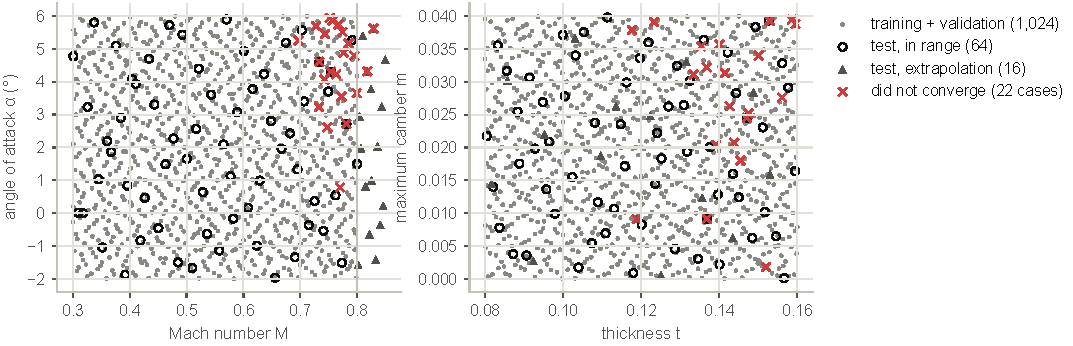
\includegraphics[width=\textwidth]{design.pdf}
\caption{The case design, projected onto two pairs of inputs. Crosses mark the 22 distinct cases
that failed the convergence rule at either grid level. All have $\Ma\ge0.697$, and 21 of the 22
have $\alpha\ge2.6^\circ$: shock-dominated cases on which the residual stalls while the forces
still move. The vertical line marks the edge of the training range, $\Ma = 0.80$.}
\label{fig:design}
\end{figure}

%===================================================================================================
\section{The learned models}
\label{sec:models}

\subsection{POD baseline}

POD needs no change of representation, because every case is the same array shape.

\paragraph{The basis.}
Stack the $N$ standardised training fields as rows of $\bm Y\in\mathbb R^{N\times D}$, with mean
$\bar{\bm y}$. The snapshot method~\cite{sirovich1987} gives the eigenpairs
$(\lambda_k,\bm v_k)$ of $(\bm Y - \bar{\bm y})(\bm Y - \bar{\bm y})^{\mathsf T}$, and from them the
orthonormal modes
\begin{equation}
  \bm\phi_k = \lambda_k^{-1/2}(\bm Y - \bar{\bm y})^{\mathsf T}\bm v_k .
\end{equation}

\paragraph{The prediction.}
A new case with inputs $\bm\mu = (\Ma,\alpha,t,m)$ is predicted as
\begin{equation}
  \hat{\bm y}(\bm\mu) = \bar{\bm y} + \sum_{k=1}^{K} a_k(\bm\mu)\,\bm\phi_k ,
\end{equation}
where each weight $a_k$ is interpolated over the inputs (scaled to the unit box) by a
thin-plate-spline radial basis function.

\paragraph{Selection.}
$K$ and the RBF smoothing were chosen on the validation set. The chosen values (256 modes,
smoothing $10^{-2}$) lie on the edges of the search grids, so the baseline may be under-tuned.

\subsection{Fourier neural operator}

\Cref{app:fno} explains the network in detail, with its tensor shapes and parameter counts.
The FNO works in the O-grid's index space. Around the airfoil the grid is periodic, so a Fourier
transform along $i$ is exact and a learned mode means the same physical wavenumber at every
resolution.

\paragraph{Inputs and outputs.}
The FNO takes six channels per node:
\begin{itemize}
  \item the radially compressed position $(x - \tfrac12,\, y)\,\ln(1+r)/r$, where $r$ is the
    distance from mid-chord;
  \item the ring index $j/(N_J-1)$;
  \item $\Ma$, $\cos\alpha$ and $\sin\alpha$, the same at every node.
\end{itemize}
The shape therefore reaches the model only through the node positions.

It predicts four channels, each of order one across the Mach range:
\begin{equation}
  \bm y = \Bigl(\hat u - \cos\alpha,\ \ \hat v - \sin\alpha,\ \ \Cp,\ \
  \frac{\hat\rho - 1}{\tfrac12\Ma^2}\Bigr).
  \label{eq:targets}
\end{equation}
Each channel is then standardised over the training set. Without this scaling, $\hat p - 1$ would
shrink like $\Ma^2$ and low-Mach cases would barely register in the loss.

\paragraph{Architecture.}
A pointwise layer lifts the six inputs to $w$ channels. Four Fourier layers follow, each
\begin{equation}
  \bm h \leftarrow \sigma\!\left(\mathcal F^{-1}\!\bigl[\bm R\cdot(\mathcal F\bm h)_{|k_i|<k_I,\ k_j<k_J}\bigr]
  + \bm W\bm h\right),
\end{equation}
with learned complex weights $\bm R$ on the retained modes, a pointwise linear path $\bm W$ and GELU
activations $\sigma$ (none after the last layer). A projection $w\to128\to4$ gives the output.

\paragraph{Radial padding.}
Radially the field is not periodic, so it is zero-padded by
\begin{equation}
  P(N_J) = \mathrm{round}\bigl(3(N_J-1)/16\bigr) - 1
\end{equation}
rows before the transform: 8 rows at $128\times49$ and 17 at $256\times97$. The discrete Fourier
period, $(N_J+P)/(N_J-1) = 19/16$ in $\eta$, is then the same at both resolutions. An earlier
padding of $(N_J-1)/6$ matched the padded span instead of the period, and one spectral layer then
differed by 4--71\,\% between the two resolutions.

\paragraph{Loss and training.}
Loss A is the per-sample relative L2 error of each output channel, averaged over channels; loss B
adds the same term on the wall row, weighted 10:
\begin{equation}
  \mathcal L_A = \frac{1}{BC}\sum_{b,c}\frac{\|\hat{\bm y}_{bc} - \bm y_{bc}\|_2}{\|\bm y_{bc}\|_2 + \epsilon},
  \qquad
  \mathcal L_B = \mathcal L_A + 10\,\mathcal L_A\big|_{j=0}.
  \label{eq:fnoloss}
\end{equation}
Training used AdamW~\cite{loshchilov2019adamw} with learning rate $10^{-3}$, cosine decay, weight
decay $10^{-4}$ and batch 8, for at most 300 epochs with early stopping at a patience of 30. It
ran on the $128\times49$ subgrid (every second node of the $256\times97$ fields), and the model is
evaluated at $256\times97$. That resolution transfer is scored separately.

\paragraph{Tuning.}
Eight configurations were trained for 100 epochs and selected on validation loss
(\cref{tab:tuning}). Width separates them; the mode counts move the loss by about as much as a
change of seed would.

\begin{table}[t]
\centering\small
\caption{FNO tuning ($n = 896$, loss A, 4 layers, 100 epochs, on the Apple GPU), and the final runs
of the selected configuration (300 epochs). Validation is relative L2 on standardised targets.}
\label{tab:tuning}
\begin{tabular}{@{}lccrr@{\hspace{8mm}}lcrrr@{}}
\toprule
\multicolumn{5}{@{}c}{Tuning} & \multicolumn{5}{c@{}}{Final runs (width 48, modes $24\times8$)}\\
\cmidrule(r{6mm}){1-5}\cmidrule{6-10}
Tag & width & modes & best val & wall s & Run & loss & best val & epoch & wall s\\
\midrule
tune-0 & 32 & $16\times8$ & 0.0315 & 419 & $n$ 896, seed 0 & A & 0.01261 & 278 & 2,160\\
tune-1 & 32 & $16\times12$ & 0.0308 & 443 & $n$ 896, seed 1 & A & 0.01274 & 293 & 2,242\\
tune-2 & 32 & $24\times8$ & 0.0310 & 443 & $n$ 896, seed 2 & A & 0.01178 & 294 & 2,237\\
tune-3 & 32 & $24\times12$ & 0.0310 & 488 & $n$ 896, seed 0 & B & 0.4617 & 50 & 605\\
tune-4 & 48 & $16\times8$ & 0.0229 & 658 & $n$ 64 & A & 0.0849 & 297 & 257\\
tune-5 & 48 & $16\times12$ & 0.0223 & 763 & $n$ 128 & A & 0.0507 & 288 & 421\\
\textbf{tune-6} & 48 & $24\times8$ & \textbf{0.0221} & 793 & $n$ 256 & A & 0.0332 & 284 & 737\\
tune-7 & 48 & $24\times12$ & 0.0235 & 859 & $n$ 512 & A & 0.0178 & 274 & 1,384\\
\bottomrule
\end{tabular}
\end{table}

\subsection{PINN}
\label{sec:pinn}

The PINN solves one test case at a time, on the same domain as SU2. It is given that case's inputs
and the O-grid map, and never any of SU2's field values. Two formulations were built. The first,
on the Euler equations, failed in a way worth recording. The second, on the full-potential
equation, is the one scored. \Cref{app:pinn} explains both in detail.

\subsubsection{The Euler PINN, and why it converges to fluid at rest}

\paragraph{Formulation.}
A fully connected tanh network takes $(\cos2\pi\xi,\ \sin2\pi\xi,\ \eta)$, which makes it periodic
around the airfoil. It outputs $\ln\rho$ and a raw velocity $\tilde{\vu}$, and two constraints are
built in:
\begin{itemize}
  \item \emph{Wall tangency}, exact by construction:
    $\vu = \tilde{\vu} - (1-\eta)^4(\tilde{\vu}\cdot\hat{\bm n}_w)\hat{\bm n}_w$.
  \item \emph{Constant total enthalpy}, so the pressure is algebraic,
    $p = \tfrac{\gamma-1}{\gamma}\rho(H_\infty - \tfrac12|\vu|^2)$ with
    $H_\infty = 1/((\gamma-1)\Ma^2) + \tfrac12$ (in $\rho_\infty U_\infty^2$ units).
\end{itemize}
The residuals of continuity and the two momentum equations are written in strong conservation form
in grid coordinates,
\begin{equation}
  \mathcal R = \frac1J\left[\frac{\partial}{\partial\xi}\bigl(y_\eta F - x_\eta G\bigr)
  + \frac{\partial}{\partial\eta}\bigl(-y_\xi F + x_\xi G\bigr)\right],\qquad
  J = x_\xi y_\eta - x_\eta y_\xi ,
  \label{eq:strongform}
\end{equation}
with the metric terms from automatic differentiation of \cref{eq:ogrid}. The free stream is a soft
penalty on the outer circle, and the Kutta condition a soft penalty on the velocity at the
trailing edge.

\paragraph{The failure.}
The warm-up is a circular cylinder at $\Ma = 0.1$, with the circulation held at zero. It must
reproduce $\Cp = 1 - 4\sin^2\theta$ to within 0.1. It failed with a largest error of 3.94: the
network had converged to \emph{fluid at rest} around the body. The wall speed was 0.004 where
potential flow gives 2.0, and $\Cp = 0.937$ everywhere (\cref{fig:warmup}).

\paragraph{Refuted hypotheses.}
Five hypotheses were each refuted by a probe:
\begin{itemize}
  \item weighting the residual by $J^p$ for $p = 0$, 0.5 and 1;
  \item an exact reparameterisation against low-Mach stiffness;
  \item a 10-chord outer boundary;
  \item a homentropic closure;
  \item the real showcase case in place of the cylinder.
\end{itemize}

\paragraph{The decisive probe.}
A network was fitted, by supervision, to the analytic potential flow. It would pass the warm-up
(shoulder speed 1.995, $\max|\Delta\Cp| = 0.030$). Yet its PINN loss is 0.31, about 1,000 times
the rest state's $\sim10^{-4}$, because small fitting errors are large derivative errors. A further
1,000 PINN-only steps from that fit drive it away from the answer.

\paragraph{Root cause.}
Fluid at rest near the body satisfies the strong-form equations and the wall condition exactly; it
violates only the weakly enforced far field. Every nearly correct flow costs more, so descent
leaves even the true solution. Within the configuration tested here the fault was in the
formulation, not in a parameter. It is not a property of Euler PINNs in general: Wassing, Langer
and Bekemeyer~\cite{wassing2025} train an Euler PINN with a soft far field to within 1\,\% of a
finite-volume reference on transonic NACA\,0012 cases (\cref{sec:discussion}).

\begin{figure}[t]
\centering
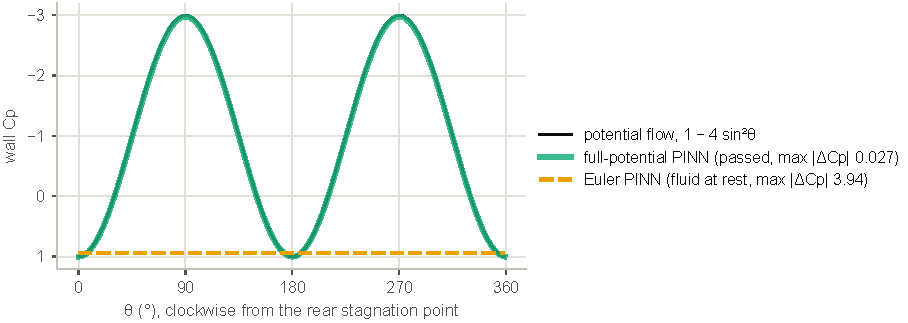
\includegraphics[width=\textwidth]{warmup.pdf}
\caption{The cylinder warm-up at $\Ma = 0.1$ (pass: $\max|\Delta\Cp|\le0.1$). The Euler PINN
reaches $\Cp\approx0.94$ all round the wall, the stagnation value: fluid at rest. The
full-potential PINN lies on the analytic curve (largest error 0.027), with $\CL$ and $\CD$ of
$-4\times10^{-4}$ and $-1\times10^{-3}$.}
\label{fig:warmup}
\end{figure}

\subsubsection{The full-potential PINN}
\label{sec:potential}

\paragraph{Formulation.}
For the full-potential equation in subcritical flow, the residual loss is (nearly) convex in the
potential, with no rest attractor, and a Dirichlet far field makes rest inadmissible. One scalar
network $\psi(\xi,\eta)$ and a learned circulation $\Gamma$ give the velocity potential, in units
of $U_\infty c$:
\begin{equation}
  \phi = x\cos\alpha + y\sin\alpha + \Gamma\,\Theta_v(x,y) + \psi(\xi,\eta)\,(1-\eta),\qquad
  \Theta_v = 1 - \frac{\operatorname{atan2}(y,\ x - \tfrac14)\bmod 2\pi}{2\pi}.
  \label{eq:phi}
\end{equation}
\begin{itemize}
  \item The factor $(1-\eta)$ vanishes on the 100-chord circle, so the far field is exact (the
    neglected doublet is $\sim10^{-3}$ there).
  \item $\Theta_v$ is the angle of a clockwise point vortex at the quarter chord. Its unit jump lies
    on the ray $y = 0$, $x > \tfrac14$, which in the domain is exactly the grid line $\xi = 0$, the
    wake cut. Its gradient, $1/(2\pi r)$, is continuous across the cut and regular at the trailing
    edge.
\end{itemize}

\paragraph{The state.}
The state follows algebraically. The velocity is $\vu = \nabla\phi$ through the metric terms,
\begin{equation}
  u = \frac{\phi_\xi y_\eta - \phi_\eta y_\xi}{J},\qquad v = \frac{-\phi_\xi x_\eta + \phi_\eta x_\xi}{J},
\end{equation}
and the density and pressure come from isentropic Bernoulli at the free-stream total enthalpy:
\begin{equation}
  \hat\rho = \Bigl[1 + \tfrac{\gamma-1}{2}\Ma^2\bigl(1 - |\vu|^2\bigr)\Bigr]^{1/(\gamma-1)},
  \qquad \hat p = \hat\rho^{\,\gamma}.
  \label{eq:bernoulli}
\end{equation}

\paragraph{The equation.}
The only equation left is steady continuity,
\begin{equation}
  \nabla\cdot(\rho\nabla\phi) = 0,
  \label{eq:fullpot}
\end{equation}
written in the strong conservation form \cref{eq:strongform} with $(F,G) = \rho(u,v)$. Momentum
holds by construction, because the flow is irrotational, isentropic and at constant $H$.
\Cref{eq:fullpot} is exact for shock-free inviscid flow and only an \emph{isentropic approximation}
at shocks. On supercritical cases it therefore solves a different equation from SU2's: there is no
entropy jump, so its shocks are those of isentropic flow.

\paragraph{Loss.}
The loss has three terms:
\begin{equation}
  \mathcal L = \underbrace{\frac{1}{N_r}\sum_{n}\mathcal R_n^2}_{\text{continuity}}
  + w_{\mathrm{wall}}\underbrace{\frac{1}{N_w}\sum_{n}(\vu\cdot\hat{\bm n}_w)^2_n}_{\partial\phi/\partial n = 0}
  + w_K\underbrace{\Bigl(|\vu|^2_{(\delta,0)} - |\vu|^2_{(1-\delta,0)}\Bigr)^2}_{\text{equal-speed Kutta}},
  \qquad w_{\mathrm{wall}} = w_K = 10.
  \label{eq:pinnloss}
\end{equation}

\paragraph{Two trailing-edge fixes.}
Both fixes were found on the first showcase case. There, the initial residual was $\sim10^5$, with
99.9\,\% of it carried by the 10 collocation points nearest the trailing edge.
\begin{enumerate}
  \item \emph{The circulation term.} It was first $\Gamma\xi$, and $|\nabla\xi|\sim r^{-1/2}$ at
    the trailing edge, where $x_\xi = y_\xi = 0$. With $\Theta_v$ the circulation-only residual
    fell from $1.2\times10^4$ to $8\times10^{-3}$.
  \item \emph{The residual near the edge.} The network term's second derivatives are singular at
    the sharp corner, as the true corner flow is. Collocation points within 0.02 chord of the
    trailing edge are therefore dropped from the residual: 197--225 of 20,000 at each resample.
\end{enumerate}

\paragraph{The Kutta condition.}
The first Kutta form, $(\partial\phi/\partial\xi)^2$ at the trailing-edge point, was degenerate.
There $x_\xi = y_\xi = 0$, so the free-stream and circulation terms contribute nothing to it, and
it could not constrain $\Gamma$. The equal-speed form in \cref{eq:pinnloss} replaces it. It
compares $|\vu|^2$ on the two surfaces at $\xi = \delta$ and $1-\delta$, with $\delta = 0.055$,
about 0.03 chord upstream of the edge.

\paragraph{Training.}
\begin{itemize}
  \item \emph{Network}: 7 hidden layers of 96 tanh units.
  \item \emph{Collocation}: 20,000 points uniform in $(\xi,\eta)$, which the map clusters near the
    wall, redrawn every 1,000 steps; 512 wall points.
  \item \emph{Adam}~\cite{kingma2015adam}: 30,000 steps in float32 on the Apple GPU, with the
    learning rate decaying exponentially from $10^{-3}$ to $10^{-4}$.
  \item \emph{L-BFGS}~\cite{liu1989lbfgs}: up to 5,000 iterations in float64 on the CPU, which has
    the float64 that the Apple GPU lacks.
\end{itemize}
One variant balances the weights by gradient norms~\cite{wang2021gradient}, every 100 steps:
\begin{equation}
  \lambda_k \leftarrow (1-a)\lambda_k + a\,\frac{\max_\theta|\nabla_\theta\mathcal L_{\mathrm{res}}|}{\overline{|\nabla_\theta\mathcal L_k|}},\qquad a = 0.9 .
  \label{eq:gradnorm}
\end{equation}

\paragraph{The runs.}
Before S3 started, every planned run was timed for a few steps. The stage refuses to start if the
projected total exceeds its budget.

Eight runs were made (\cref{tab:pinnruns}):
\begin{itemize}
  \item the six showcase cases with fixed weights (\texttt{pure});
  \item gradient-norm balancing on the median-Mach case (\texttt{gradnorm});
  \item one run without the Kutta term (\texttt{nokutta}), for prediction P3.
\end{itemize}

The specification also called for runs with an artificial viscosity at shocks, $\nu = 10^{-3}$ and
$3\times10^{-4}$. They were dropped by the author's decision of 5 October 2026: at about a day each,
the four of them would have added roughly 46 hours on two shards.

\begin{table}[t]
\centering\small
\caption{The eight PINN runs (stage S3). Two runs shared the machine at a time, which inflates the
mean wall time by at most about 1.2 times. Losses are the final values after L-BFGS.}
\label{tab:pinnruns}
\begin{tabular}{@{}llrrrrrr@{}}
\toprule
Variant & Case (regime) & Wall h & CPU h & Residual & Wall & Kutta & Total\\
\midrule
pure & 0022 (sub) & 5.45 & 9.74 & $2.25\times10^{-3}$ & $1.3\times10^{-4}$ & $1.2\times10^{-7}$ & $3.58\times10^{-3}$\\
pure & 0021 (sub) & 5.33 & 9.27 & $4.91\times10^{-3}$ & $3.9\times10^{-4}$ & $5.9\times10^{-6}$ & $8.92\times10^{-3}$\\
pure & 0043 (sub) & 4.97 & 9.23 & $1.10\times10^{-3}$ & $4.9\times10^{-5}$ & $8.8\times10^{-8}$ & $1.59\times10^{-3}$\\
pure & 0004 (super) & 5.01 & 9.40 & $2.98\times10^{-3}$ & $2.2\times10^{-4}$ & $1.2\times10^{-7}$ & $5.15\times10^{-3}$\\
pure & 0031 (super) & 6.47 & 11.57 & $5.31\times10^{-3}$ & $4.2\times10^{-4}$ & $4.5\times10^{-7}$ & $9.50\times10^{-3}$\\
pure & 0040 (super) & 6.44 & 11.56 & $2.38\times10^{-2}$ & $2.1\times10^{-3}$ & $5.7\times10^{-6}$ & $4.51\times10^{-2}$\\
nokutta & 0022 (sub) & 5.40 & 10.08 & $1.82\times10^{-3}$ & $7.8\times10^{-5}$ & 0 & $2.61\times10^{-3}$\\
gradnorm & 0004 (super) & 4.96 & 7.20 & 9.11 & $9.4\times10^{-3}$ & $1.9\times10^{-13}$ & 82.2\\
\bottomrule
\end{tabular}
\end{table}

%===================================================================================================
\section{Scoring}
\label{sec:scoring}

\paragraph{Truth and the floor.}
The truth is SU2 on the $512\times193$ grid, read at every second node. Because the grids nest,
those nodes are exactly the $256\times97$ nodes, and every contestant is evaluated on them. The
floor is SU2's $256\times97$ solution scored against that truth. It is the error that being on the
evaluation grid already costs, so a surrogate at the floor is as good as SU2 on that grid.

\paragraph{One force integrator.}
The integration is vertex-lumped: each wall node carries half of each adjacent edge's outward
normal,
$\bm n_i = \tfrac12(\bm n_{e,i-1} + \bm n_{e,i})$. With $\bm f = -\sum_i \Cp{}_{,i}\,\bm n_i$, the
coefficients are
\begin{equation}
  \CD = f_x\cos\alpha + f_y\sin\alpha,\qquad
  \CL = -f_x\sin\alpha + f_y\cos\alpha,\qquad
  \CM = \sum_i\bigl[(x_i - \tfrac14)f_{y,i} - y_i f_{x,i}\bigr].
  \label{eq:forces}
\end{equation}
On SU2's own solutions this reproduces SU2's reported coefficients to $5\times10^{-11}$. The
edge-midpoint trapezoid matched $\CL$ and $\CD$ but missed $\CM$ by $1.6\times10^{-5}$, which fails
the $10^{-6}$ check.

\paragraph{Errors.}
Force errors are absolute, with $\CD$ in counts, because percentages of near-zero inviscid drag mean
nothing. The wall-pressure error is the RMS of $\Delta\Cp$ over the wall nodes. The near-field
error is the area-weighted relative L2 error over the nodes within 2.5 chords of mid-chord:
\begin{equation}
  e_{\mathrm{nf}} = \left(\frac{\sum_{i}w_i\,|\hat{\bm q}_i - \bm q_i|^2}{\sum_i w_i\,|\bm q_i - \bm q_\infty|^2}\right)^{1/2},
  \qquad |\bm x_i - (\tfrac12,0)|\le2.5,
  \label{eq:nearfield}
\end{equation}
where $w_i$ is the dual-cell area.

\paragraph{Shocks.}
On each surface that goes supersonic, the shock is the steepest pressure rise downstream of the
suction peak, among segments whose upstream node is supersonic. Without that restriction the rule
finds the trailing-edge recompression on every real solution. The overshoot is the largest
$|\Delta\Cp|$ within 0.05 chord of the true shock.

\paragraph{Physics checks.}
These run on every column, SU2 included:
\begin{itemize}
  \item the entropy in subcritical cases;
  \item $|H/H_\infty - 1|$;
  \item the RMS velocity through the wall;
  \item the net mass flux through the closed grid lines $j = 8$, 24, 48 and 72.
\end{itemize}
A check that a contestant satisfies by construction is labelled as such. For the potential PINN,
entropy and enthalpy are identities, and wall tangency is a result.

\paragraph{Cost.}
Each method's cost is a fixed part plus a part per new case,
\begin{equation}
  C_m(n) = C_m^{\mathrm{fixed}} + n\,c_m,\qquad
  n^\ast_m = \min\{n : C_m(n) < n\,c_{\mathrm{SU2}}\}.
  \label{eq:breakeven}
\end{equation}
\begin{itemize}
  \item SU2's cost per case is its median CPU time on the test cases.
  \item The fixed cost of the FNO and of POD is the whole campaign, every validation case included,
    plus model search and final training.
  \item GPU work is charged at wall time, because process CPU time cannot see it; CPU work is
    charged at CPU time. The PINN is charged per phase: Adam (GPU) at wall time, L-BFGS (CPU) at
    CPU time.
\end{itemize}

%===================================================================================================
\section{Results}
\label{sec:results}

\subsection{The three predictions}
\label{sec:predictions}

\begin{table}[t]
\centering\small
\caption{The predictions recorded before any model ran, and their outcomes.}
\label{tab:predictions}
\begin{tabularx}{\textwidth}{@{}>{\raggedright\arraybackslash}p{0.35\textwidth}>{\raggedright\arraybackslash}X@{}}
\toprule
Prediction & Outcome\\
\midrule
P1. For a single new case, SU2 beats the PINN on cost by one to two orders of magnitude. &
\textbf{Held on wall time only} (88.5$\times$, 1.95 orders). \textbf{Not held} on CPU time or
per phase (174--220$\times$, 2.24--2.34 orders): SU2 wins by more than predicted.\\
\addlinespace
P2. The FNO beats ``just run SU2'' only after about as many new cases as trained it ($\sim$1,000). &
\textbf{Held.} Break-even at $n^\ast = 1{,}126$ new cases. The data-efficiency curve is still
3.4$\times$ the floor at $n = 896$, so the ``unless'' clause does not fire.\\
\addlinespace
P3. Without the Kutta condition the PINN's residuals look acceptable while its lift is wrong. &
\textbf{Partly.} Without the condition the residual is as small as with it ($1.8\times10^{-3}$
against $2.3\times10^{-3}$) and the lift is 84\,\% low. But with the condition it is still 77\,\%
low: the Kutta term made no material difference to the circulation.\\
\bottomrule
\end{tabularx}
\end{table}

\Cref{tab:predictions} gives the verdicts. The costs behind P1 are in \cref{tab:costs}.

\paragraph{P1 depends on the cost basis.}
The mean \texttt{pure} run took 20,201\,s of wall time and 36,464\,s of CPU time, because L-BFGS
ran multithreaded on the CPU. SU2 took a median 228.1\,s of wall time and 209.9\,s of CPU time per
case.
\begin{itemize}
  \item Wall time against wall time gives 88.5$\times$, inside the predicted band.
  \item The per-phase rule, which the scorer applies to every other method, gives 174--220$\times$,
    outside it.
\end{itemize}
The per-phase cost is a bracket, not a single figure, because the S3 runs did not record the Adam
phase's own CPU time. A later measurement of that fraction (0.346) gives 204$\times$.

\begin{table}[t]
\centering\small
\caption{Costs, in seconds. SU2 per case is the median over the 80 test cases at $256\times97$.
The FNO and POD fixed costs include the full campaign (229,211\,s of CPU time). The PINN has no
fixed cost.}
\label{tab:costs}
\begin{tabularx}{\textwidth}{@{}lrrr>{\raggedright\arraybackslash}X@{}}
\toprule
Method & Fixed & Per case (wall) & Per case (CPU) & Basis used for break-even\\
\midrule
SU2 $256\times97$ & 0 & 228.1 & 209.9 & CPU, 209.9\\
FNO & 236,237 & \multicolumn{2}{c}{0.054 per query} & campaign + 8 tuning runs (4,867) + training (2,160)\\
POD & 229,562 & \multicolumn{2}{c}{0.007 per query} & campaign + mode and smoothing search\\
PINN (\texttt{pure}, mean of 6) & 0 & 20,201 & 36,464 & per phase: 36,464--46,122\\
\bottomrule
\end{tabularx}
\end{table}

\subsection{Accuracy by regime and set}

\Cref{tab:results} and \cref{fig:nearfield} give the main result, with the floor beside every error.

\begin{table}[t]
\centering\small
\caption{Errors by set and regime, with the floor first. Near field: mean of
\cref{eq:nearfield}; $\CL$ and $\CD$: largest absolute error in the group; $\Cp$: mean RMS wall
error. FNO rows are seed 0, $n = 896$, loss A, scored on its $256\times97$ evaluation grid and on
its $128\times49$ training grid (against the truth at every fourth fine node). PINN rows cover the
three showcase cases of each regime.}
\label{tab:results}
\begin{tabular}{@{}llrrrr@{}}
\toprule
Set / regime & Method & Near field & $\CL$ max & $\CD$ max (counts) & $\Cp$ RMS\\
\midrule
\multirow{5}{*}{\shortstack[l]{in range\\subcritical (37)}}
 & \textbf{floor} & \textbf{0.0080} & \textbf{0.0073} & \textbf{6.9} & \textbf{0.0357}\\
 & FNO $256\times97$ & 0.0423 & 0.0312 & 31.3 & 0.0358\\
 & FNO $128\times49$ & 0.0102 & 0.0095 & 7.5 & 0.0334\\
 & POD & 0.0168 & 0.0097 & 14.2 & 0.0371\\
 & PINN (3) & 0.5155 & 0.2461 & 41.1 & 0.1603\\
\midrule
\multirow{5}{*}{\shortstack[l]{in range\\supercritical (24)}}
 & \textbf{floor} & \textbf{0.0241} & \textbf{0.0140} & \textbf{17.2} & \textbf{0.0341}\\
 & FNO $256\times97$ & 0.0575 & 0.0431 & 40.4 & 0.0521\\
 & FNO $128\times49$ & 0.0374 & 0.0314 & 46.6 & 0.0470\\
 & POD & 0.1462 & 0.0750 & 122.2 & 0.1190\\
 & PINN (3) & 0.6273 & 1.4028 & 776.5 & 0.4045\\
\midrule
\multirow{4}{*}{\shortstack[l]{extrapolation\\supercritical (14)}}
 & \textbf{floor} & \textbf{0.0651} & \textbf{0.0247} & \textbf{32.4} & \textbf{0.0598}\\
 & FNO $256\times97$ & 0.2318 & 0.1847 & 180.6 & 0.2038\\
 & FNO $128\times49$ & 0.2320 & 0.1876 & 178.3 & 0.1966\\
 & POD & 0.5151 & 0.3483 & 530.2 & 0.3512\\
\bottomrule
\end{tabular}
\end{table}

\begin{figure}[t]
\centering
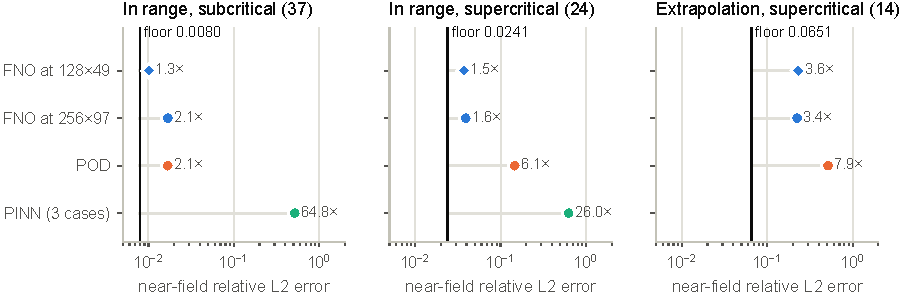
\includegraphics[width=\textwidth]{nearfield.pdf}
\caption{Near-field error against the floor (vertical line); each label is the ratio to the floor.
The FNO at $128\times49$ is scored on its own training grid, so its comparison grid is coarser
than the floor's.}
\label{fig:nearfield}
\end{figure}

What the table says:
\begin{itemize}
  \item \textbf{In range and subcritical, the FNO at its own resolution is near the floor}: 1.3
    times on the near field, 1.3 times on $\CL$ and 1.1 times on $\CD$. Evaluated at
    $256\times97$ it is 5.3 times the floor, and POD beats it there on the near field, $\CL$ and
    $\CD$. The resolution transfer costs the FNO more than any other single factor in range.
  \item \textbf{In range and supercritical, the FNO beats POD by 2.5 times} on the near field and 3
    times on $\CD$, at 2.4 times the floor. Shocks that move with the inputs are exactly where a
    fixed linear basis struggles.
  \item \textbf{Extrapolation is where every surrogate fails.} The FNO is 3.6 times the floor, and
    its $\CD$ error reaches 181 counts, biased rather than scattered (median $-78$ counts); POD is
    7.9 times the floor. Here the FNO is equally wrong at both resolutions.
  \item \textbf{The PINN is not competitive in any column}: 65 and 26 times the floor on the near
    field.
\end{itemize}

\subsection{Fields and wall pressure}

\Cref{fig:fields} shows the Mach field of one subcritical and one supercritical case from each
method.
\begin{itemize}
  \item On the subcritical case the FNO and POD are close to the truth at this scale. The PINN's
    field is nearly symmetric about the chord: the faster flow over the upper surface, which
    carries the lift, is missing.
  \item On the strongest supercritical showcase case (\texttt{test\_in-0040}, maximum surface
    Mach 1.61) the FNO places the supersonic pocket and its terminating shock well. POD shrinks the
    pocket and moves the shock forward. The PINN has no supersonic region at all: its lift on this
    case is $-0.015$, against SU2's 1.388.
\end{itemize}
\Cref{fig:showcase} gives the wall pressure on all six showcase cases.

\begin{figure}[t]
\centering
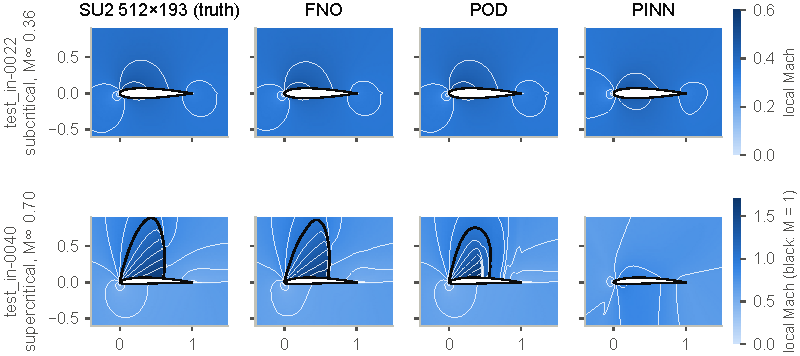
\includegraphics[width=\textwidth]{fields.pdf}
\caption{Local Mach number near the section: the truth and each contestant. Thin white lines are
iso-Mach contours (every 0.05 in the top row, 0.1 in the bottom); the black line is the sonic line.
Each row has its own colour scale.}
\label{fig:fields}
\end{figure}

\begin{figure}[t]
\centering
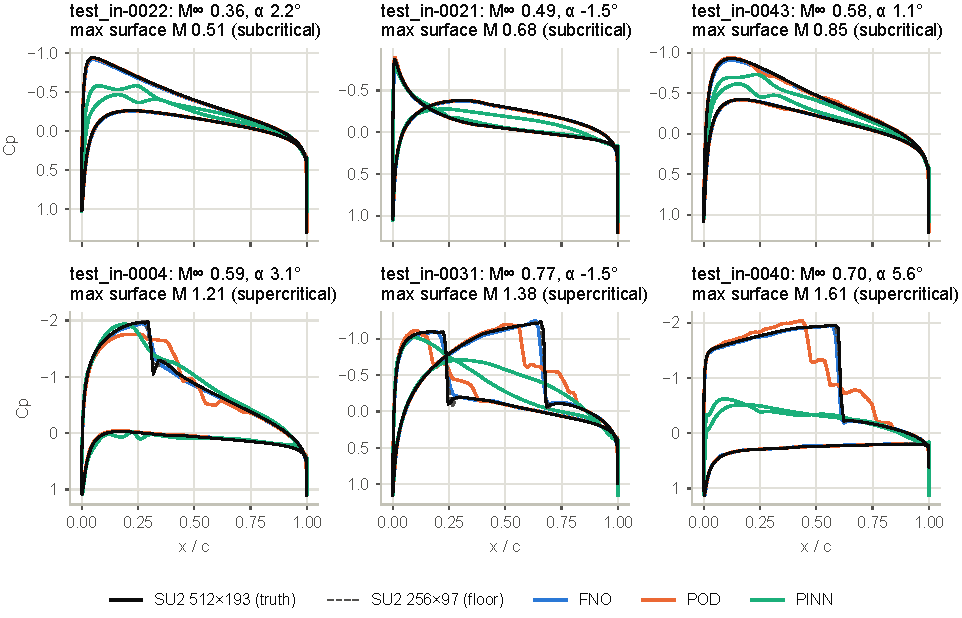
\includegraphics[width=\textwidth]{showcase.pdf}
\caption{Wall pressure on the six showcase cases, in order of maximum surface Mach number
($\Cp$ axis inverted). The floor lies under the truth everywhere. The FNO follows the truth closely
and smears the shocks a little. POD's shocks are displaced and broken into steps. The PINN's
suction peaks are too weak, the signature of a circulation far below the Kutta value.}
\label{fig:showcase}
\end{figure}

\subsection{Lift}

The PINN's lift error is the clearest failure (\cref{fig:clparity}, \cref{tab:pinncl}). Five of the
six \texttt{pure} runs under-predict lift, three of them to roughly zero. By Kutta--Joukowski,
$L' = \rho_\infty U_\infty\Gamma$, so $\Gamma = \CL/2$ in units of $U_\infty c$; a lift 4.4 times
too small on \texttt{test\_in-0022} is a circulation 4.4 times too small.

\paragraph{The Kutta term can pin $\Gamma$.}
The equal-speed term does pin the circulation of a true potential flow. On the exact
incompressible flat-plate (Joukowski) flow at $\alpha = 2.19^\circ$, evaluated 0.03 chord upstream
of the trailing edge, the quantity $|\vu|^2_{\mathrm{upper}} - |\vu|^2_{\mathrm{lower}}$ is:
\begin{itemize}
  \item $-0.421$ at $\Gamma = 0$;
  \item $-0.277$ at $\Gamma = 0.0387$, the value recovered for the \texttt{pure} run;
  \item $+0.027$ at the Kutta value $\Gamma = \pi\sin\alpha = 0.120$.
\end{itemize}

\paragraph{So the network is not a potential flow near the edge.}
A wrong-$\Gamma$ potential flow would pay about 100 times the penalty of the right one. A network
that meets the term to $10^{-7}$ at the wrong $\Gamma$ is therefore not a potential-flow solution
near the trailing edge. Whether the network's representation, the 0.02-chord exclusion or both is
responsible is not isolated here.

\begin{figure}[t]
\centering
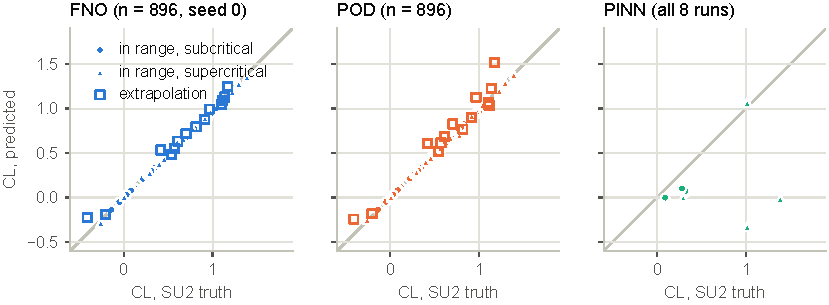
\includegraphics[width=\textwidth]{cl_parity.pdf}
\caption{Predicted against true $\CL$ at $256\times97$. Filled markers: in range; hollow:
extrapolation. In extrapolation the FNO's lift errors reach $+0.18$ and POD's $+0.35$, and POD
over-predicts at the median ($+0.06$). The PINN's points lie well below it, except \texttt{pure} on
\texttt{test\_in-0004}. The \texttt{gradnorm} run on that case is at $(1.01,\,-0.33)$.}
\label{fig:clparity}
\end{figure}

\begin{table}[t]
\centering\small
\caption{The PINN per case (test\_in, $256\times97$). The floor's $\CL$ errors on these cases are
0.0003--0.0086.}
\label{tab:pinncl}
\begin{tabular}{@{}llrrrrr@{}}
\toprule
Run & Regime & SU2 $\CL$ & PINN $\CL$ & $\CL$ error & $\CD$ error (counts) & Near field\\
\midrule
pure / 0022 & sub & 0.3192 & 0.0732 & $-0.2461$ & $+41.1$ & 0.559\\
nokutta / 0022 & sub & 0.3192 & 0.0526 & $-0.2667$ & $+30.0$ & 0.569\\
pure / 0021 & sub & 0.0922 & $-0.0012$ & $-0.0934$ & $-5.6$ & 0.629\\
pure / 0043 & sub & 0.2799 & 0.1008 & $-0.1790$ & $+15.1$ & 0.359\\
pure / 0004 & super & 1.0139 & 1.0662 & $+0.0523$ & $+88.6$ & 0.218\\
pure / 0031 & super & 0.2949 & 0.0007 & $-0.2942$ & $-9.9$ & 0.584\\
pure / 0040 & super & 1.3879 & $-0.0149$ & $-1.4028$ & $-776.5$ & 1.080\\
gradnorm / 0004 & super & 1.0139 & $-0.3272$ & $-1.3411$ & $+724.8$ & 1.273\\
\bottomrule
\end{tabular}
\end{table}

\subsection{PINN training}

\paragraph{The loss does not reveal the circulation.}
\Cref{fig:pinnhistory}(a) shows that the residual loss converges equally well with and without the
Kutta term.

\paragraph{The gradnorm run.}
Gradient-norm balancing failed in a specific way (\cref{fig:pinnhistory}(b)):
\begin{itemize}
  \item From step 500 on, the weighted wall term was at least 96\,\% of the total at every logged
    step, while the balanced wall weight ranged from 692 to $1.3\times10^5$.
  \item The wall loss itself stayed at 0.03--0.25, 33 times the fixed-weight run's at the end of
    Adam.
  \item L-BFGS then minimised an objective that was 99.99\,\% wall term. It cut the wall loss
    tenfold and made the equation residual 380 times worse, from 0.024 to 9.11.
\end{itemize}
The run's lift has the wrong sign. The Kutta weight also ran away, to a logged peak of
$7\times10^{10}$, but it multiplied a Kutta loss below $10^{-9}$ and barely moved the total.

\begin{figure}[t]
\centering
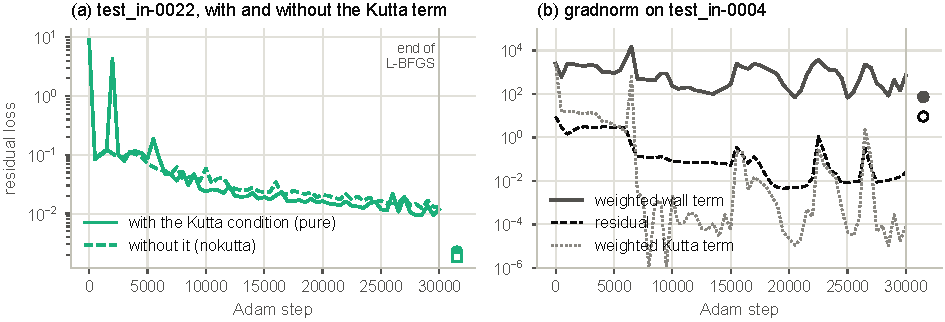
\includegraphics[width=\textwidth]{pinn_history.pdf}
\caption{PINN training histories (logged every 500 Adam steps; markers right of the line: after
L-BFGS). (a) With and without the Kutta term on the same case: indistinguishable losses, both with
lift far too low. (b) The \texttt{gradnorm} run: the balanced wall term dominates the objective,
and L-BFGS trades the residual for it.}
\label{fig:pinnhistory}
\end{figure}

\subsection{FNO: seeds, loss B and shocks}

\paragraph{Seeds.}
Across the three seeds at $n = 896$, the near field varies by a few per cent of its value. The
extrapolation $\CL$ maximum, however, varies by 40\,\% (0.173--0.243), so a single-seed
extrapolation lift figure is not reliable to better than that.

\paragraph{Loss B.}
Loss B is worse than loss A on the near field and $\CD$ in every set and regime, at both grids. It
is worse on $\CL$ in every cell but one: in-range subcritical at $256\times97$, where it is 23\,\%
better. It is worst on supercritical lift ($\CL$ maximum 0.249 against 0.043). It stopped early, at
epoch 81, so this compares the runs as made, not converged runs.

\paragraph{Shocks.}
\Cref{tab:shocks} gives the shock scores.
\begin{itemize}
  \item In range, the FNO places shocks at the floor's median accuracy but misses 1--2 of 27 and
    smears them, with twice the floor's median overshoot.
  \item POD never misses a shock but places them 0.06--0.11 chord off at the median.
  \item Out of range, the FNO's position errors reach 0.21 chord.
\end{itemize}

\begin{table}[t]
\centering\small
\caption{Shocks: 27 true shocks on the 24 in-range supercritical cases and 21 on the 14
extrapolation cases. Position error in chords; overshoot is the largest $|\Delta\Cp|$ within 0.05
chord of the true shock.}
\label{tab:shocks}
\begin{tabular}{@{}llrcc@{}}
\toprule
Set & Method & Missed & $|\Delta x|$ median / max & Overshoot median / max\\
\midrule
in range & \textbf{floor} & \textbf{0} & \textbf{0 / 0.019} & \textbf{0.19 / 0.54}\\
 & FNO $256\times97$ & 2 & 0 / 0.058 & 0.42 / 1.05\\
 & FNO $128\times49$ & 1 & 0 / 0.069 & 0.29 / 0.92\\
 & POD & 0 & 0.061 / 0.135 & 0.65 / 1.34\\
 & FNO loss B & 2 & 0.012 / 0.068 & 0.59 / 1.29\\
 & PINN \texttt{pure} (3 cases, 4 shocks) & 1 & 0.046 / 0.181 & 0.74 / 1.67\\
\midrule
extrapolation & \textbf{floor} & \textbf{0} & \textbf{0.008 / 0.012} & \textbf{0.69 / 1.00}\\
 & FNO $256\times97$ & 0 & 0.042 / 0.213 & 1.13 / 1.58\\
 & POD & 0 & 0.106 / 0.250 & 1.28 / 1.60\\
\bottomrule
\end{tabular}
\end{table}

\subsection{Data efficiency and break-even}

\Cref{fig:efficiency} and \cref{tab:efficiency} show the test error against the number of SU2 cases
paid for. Both models are still improving at $n = 896$, and neither approaches the floor. A smaller
training set would break even sooner, at about 199 cases for $n = 64$, but its answers would be 7.6
times the floor rather than 3.4. \Cref{fig:breakeven} draws \cref{eq:breakeven}: the FNO and POD
lines cross SU2's at 1,126 and 1,094 new cases.

\begin{table}[t]
\centering\small
\caption{Data efficiency: mean near-field error over the 61 in-range test cases at $256\times97$
(floor 0.0143), with the SU2 cost paid for each training set (every validation case included).}
\label{tab:efficiency}
\begin{tabular}{@{}rrrrrr@{}}
\toprule
$n$ & FNO (seed 0) & FNO / floor & POD & POD / floor & Campaign, SU2-case equivalents\\
\midrule
64 & 0.1088 & 7.6$\times$ & 0.1379 & 9.6$\times$ & 197\\
128 & 0.0858 & 6.0$\times$ & 0.1044 & 7.3$\times$ & 257\\
256 & 0.0698 & 4.9$\times$ & 0.0883 & 6.2$\times$ & 380\\
512 & 0.0561 & 3.9$\times$ & 0.0753 & 5.3$\times$ & 690\\
896 & 0.0483 & 3.4$\times$ & 0.0677 & 4.7$\times$ & 1,092\\
\bottomrule
\end{tabular}
\end{table}

\begin{figure}[t]
\centering
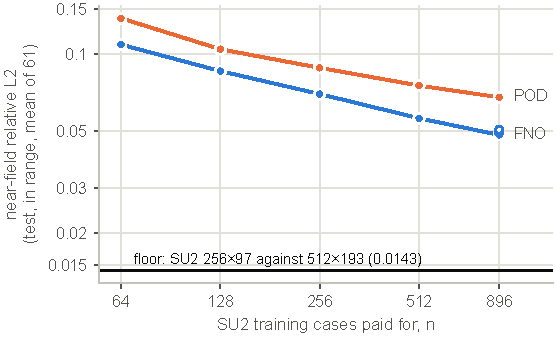
\includegraphics[width=0.66\textwidth]{efficiency.pdf}
\caption{Data efficiency. Open markers at $n = 896$ are the FNO's seeds 1 and 2.}
\label{fig:efficiency}
\end{figure}

\begin{figure}[t]
\centering
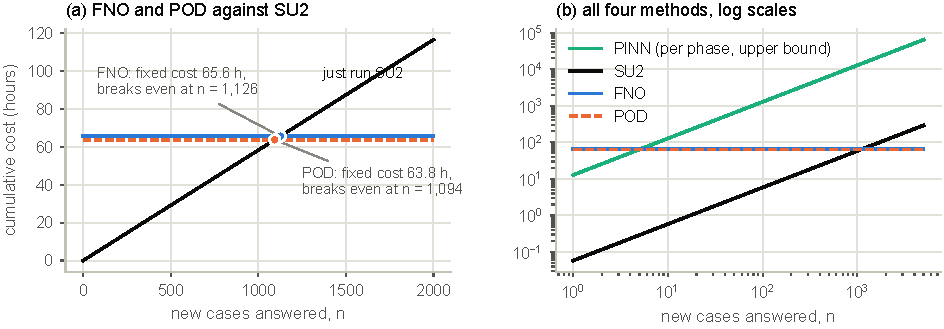
\includegraphics[width=\textwidth]{break_even.pdf}
\caption{Cumulative cost of answering $n$ new cases. (a) The FNO and POD each pay roughly a whole
campaign up front (65.6 and 63.8 hours) and break even after about as many new cases as the
campaign held. (b) The PINN, at 12.8 hours per case (per-phase upper bound), is above SU2 at every
$n$, above POD from the fifth case and above the FNO from the sixth.}
\label{fig:breakeven}
\end{figure}

\subsection{Physics checks and failures}

\paragraph{SU2 itself.}
SU2 is not free of numerical artefacts:
\begin{itemize}
  \item \emph{Entropy.} In subcritical cases, where it should be zero, the truth's near-field
    maximum entropy has median 0.020, and the floor's 0.033, so SU2 generates spurious entropy, and
    more of it on the coarser grid. Its area-weighted mean is small and non-negative on every case
    at both grids.
  \item \emph{Total enthalpy} is constant to $1.2\times10^{-5}$.
  \item \emph{No} non-positive density or pressure appears anywhere.
\end{itemize}

\paragraph{Failures, stated as results.}
\begin{itemize}
  \item \emph{Non-physical states in extrapolation.} POD predicts non-positive density or pressure
    on 2 to 7 of the 14 extrapolation cases, and more as the training set grows. The FNO does so on
    4--5 cases at $n\le128$ and on none at $n\ge256$.
  \item \emph{Entropy decrease.} The subcritical near-field mean entropy falls below free stream on
    9--24 of 37 cases for the FNO and 10--23 for POD, against none for SU2. Whether any surrogate
    predicts an expansion shock is not measured: the scorer has no test for an entropy decrease
    across a compression.
  \item \emph{PINN wall tangency and mass.} The potential PINN enforces both only softly: its RMS
    wall-normal velocity has median 0.011 (subcritical) and 0.020 (supercritical), against SU2's
    $10^{-8}$. Its mass flux through the closed lines is one to two orders above the FNO's.
  \item \emph{Not measured}: FNO ringing (only the plots show it), and the viscous PINN (dropped
    from S3; the artificially viscous PINN of S5 is in \cref{sec:s5}).
\end{itemize}

%===================================================================================================
\clearpage
\section{Stage S5: a published Euler PINN, rebuilt}
\label{sec:s5}

Wassing, Langer and Bekemeyer~\cite{wassing2025} report an Euler PINN that captures the shock on
transonic NACA\,0012 cases to within 0.3--0.4\,\% in Cp (\cref{sec:discussion}). This study's own
Euler PINN converged to fluid at rest. Stage S5 rebuilt their recipe from the paper, on this
study's grid, and asked three questions in turn:
\begin{enumerate}
  \item Does the rebuilt recipe pass a validation gate against SU2 on their case B?
  \item If it does, which of its ingredients does it need? (A one-at-a-time ablation.)
  \item How does it compare with the FNO on three in-range and three extrapolation cases?
\end{enumerate}
Four predictions were recorded before any S5 code existed (\cref{tab:s5predictions}). The design
fixes what happens if the gate fails: S5 stops after step 1. It did.

\subsection{The recipe as built}
\label{sec:s5recipe}

\paragraph{State and network.}
The network outputs the primitive variables $(\rho,u,v,p)$ in their scaling: $\rho_\infty =
p_\infty = 1$ and $\vu_\infty = \sqrt{\gamma}\,\Ma(\cos\alpha,\sin\alpha)$, so $c_\infty =
\sqrt\gamma$. Its input is the index pair $\bm r = (i,j)$ of the $512\times193$ collocation grid,
through random Fourier features,
\begin{equation}
  \bm\gamma(\bm r) = \bigl[\sin(\Phi\bm r),\ \cos(\Phi\bm r)\bigr],\qquad
  \Phi\in\mathbb R^{128\times2},\quad \Phi_{kl}\sim\mathcal N(0,1),
  \label{eq:fourierfeatures}
\end{equation}
followed by five weight-normalised layers of 128 units. Each layer $k$ has a layer-wise adaptive
activation $\sigma_k(x) = \tanh(n\,\omega_k x)$, with $\omega_k$ trained. Their scale factor $n$ is
not stated; here $n = 10$ and $\omega_k$ starts at 0.1, following Jagtap et
al.~\cite{jagtap2020}, so that $n\omega_k = 1$ at the start. A last weight-normalised affine map
gives the four outputs.

\paragraph{Loss.}
Collocation is at every node of the grid, in mini-batches of 5,000:
\begin{gather}
  L = \lambda_{\mathrm{res}} L_{\mathrm{res}} + L_\infty + L_{\mathrm{af}} + L_{\mathrm{lr}},\qquad
  L_{\mathrm{res}} = \frac1{N_b}\sum_{n\in\text{batch}} w_n\,\bigl|\nabla\!\cdot\!\bm F(W_n) - D(W_n)\bigr|^2,
  \label{eq:s5loss}
\end{gather}
with $\lambda_{\mathrm{res}} = 2\times10^4$. The weight $w_n$ is the node's dual-cell area,
normalised to mean 1 over the grid (their volume weighting). $L_\infty$, $L_{\mathrm{af}}$ and
$L_{\mathrm{lr}}$ are mean squares of the far-field mismatch $\hat q - w_\infty$ on the outer row,
of the wall-normal velocity $\vu\cdot\hat{\bm n}$ on the wall row, and of the periodicity
mismatch across the cut.

\paragraph{Artificial viscosity.}
The viscous term acts on the density and energy equations only, through the selector
$I_{\rho,\rho E} = \mathrm{diag}(1,0,0,1)$:
\begin{equation}
  D = \mu_x\frac{\partial^2 W}{\partial x^2} + \mu_y\frac{\partial^2 W}{\partial y^2},\qquad
  \mu_x = \nu\,s\,I_{\rho,\rho E}\,|A|,\quad \mu_y = \nu\,s\,I_{\rho,\rho E}\,|B|,\qquad \nu = 1.9\times10^{-3}.
  \label{eq:s5visc}
\end{equation}
Here $|A| = T|\Lambda|T^{-1}$ is the absolute flux Jacobian, in Swanson and Turkel's closed
form~\cite{swanson1992}, with each eigenvalue limited below at 0.25. The sensor
\begin{equation}
  \begin{gathered}
  s = s_{\mathrm{shock}}\,s_{\mathrm{stag}},\qquad
  s_{\mathrm{shock}} = \tanh\Bigl(\max\bigl(0,\ k^{(1)}_{\mathrm{shock}}\,\tfrac{\vu}{|\vu|}\cdot\nabla p - k^{(0)}_{\mathrm{shock}}\bigr)\Bigr),\\
  s_{\mathrm{stag}} = \mathrm{sig}\Bigl(k^{(1)}_{\mathrm{stag}}\bigl(k^{(0)}_{\mathrm{stag}} - |\nabla(\rho u)| - |\nabla(\rho v)|\bigr)\Bigr),\qquad
  k^{(0)}_{\mathrm{stag}} = 3,\quad k^{(1)}_{\mathrm{stag}} = 5,
  \end{gathered}
  \label{eq:s5sensor}
\end{equation}
is detached from the gradient graph. It switches the viscosity on where the pressure rises along
the flow, and off at stagnation points. Their table gives the two shock constants in an ambiguous
form, so both readings were kept as tuning configurations. Their Eq.~(13) writes the residual as
$\nabla\!\cdot\!\bm F + D$, which with \cref{eq:s5visc} is anti-dissipative. The sign used here,
$\nabla\!\cdot\!\bm F - D$, is the dissipative one, read as their intent.

\paragraph{Optimiser.}
Each mini-batch gets a fresh L-BFGS (at most 1,000 iterations and 1,250 evaluations, a history of
1,000, strong-Wolfe line search), reset after its outer iteration. There are 20 batches per epoch
and 40 epochs: 800 outer iterations.

\paragraph{Departures, declared before any run.}
The grid is this study's algebraic O-grid with its 100-chord radius and $512\times193$ nodes,
because the truth lives on it; theirs is a $400\times200$ elliptic grid. The metric terms come
from automatic differentiation of the analytic map. The trailing-edge wall node, where the map's
Jacobian vanishes, is left out of the residual. The boundary terms are evaluated in full at every
closure.

\paragraph{The gate and its tuning budget.}
The gate is their error metric~\cite[Eq.~28]{wassing2025}: the relative mean absolute error
$\mathrm{RMAE} = \mathrm{MAE}/(\max u - \min u)$, of Cp and of local Mach number. It is evaluated
on a $401\times401$ lattice over $x\in[-0.5,1.5]$, $y\in[-1,1]$, against SU2 at $512\times193$.
Both must be at most 1\,\%. Four configurations make the tuning budget, each changing one thing
from T1, the recipe as specified: T2 takes the other reading of the shock constants, T3 the scalar
viscosity $\mu = \nu s\,I_{\rho,\rho E}(c+|\vu|)$, and T4 a 0.02-chord exclusion around the
trailing edge. The first configuration to pass becomes the recipe R that steps 2 and 3 use. Before
each configuration trains, one real epoch of it is timed; the run is projected at 40 times that,
and the gate refuses it if the projection would carry the gate past 72\,h.

\subsection{Before the gate: a uniform field}
\label{sec:s5trap}

A probe run before launch found the failure the gate later measured. One epoch of T1 on case B
took the loss from 279.6 to 0.0508 in the first outer iteration, in 97 closures. In that step the
fourth layer's slope went to $\omega_4 = 0$. With $\tanh(0) = 0$, that layer outputs zero for
every input, so the network is a constant, and the field is uniform to $3\times10^{-8}$. A uniform
stream satisfies the Euler equations exactly and makes the viscous term vanish, so its loss is the
wall-tangency term alone, $\overline{(\vu\cdot\hat{\bm n})^2}\approx 0.047$, plus a small far-field
term. Every way out runs through the dead layer's pre-activations. Those are random and vary from
cell to cell, so no Euler solution resembles them, and each costs far more residual than it saves
at the wall. The remaining 19 outer iterations stalled after 3--5 closures each.

\begin{table}[t]
\centering\small
\caption{Where the weighted residual sits at initialisation (T1, case B, every residual node).
$\lambda_{\mathrm{res}}L_{\mathrm{res}} = 235.7$ against $L_\infty+L_{\mathrm{af}}+L_{\mathrm{lr}}
= 2.52$.}
\label{tab:s5split}
\begin{tabular}{@{}lrr@{}}
\toprule
Region & Share of nodes & Share of $\lambda_{\mathrm{res}}L_{\mathrm{res}}$\\
\midrule
Wall rows, $j<10$ & 5.2\,\% & 42.9\,\%\\
Rest of the gate's box & 37.8\,\% & 42.8\,\%\\
Outer rows, $j\ge183$ & 5.2\,\% & 1.3\,\%\\
Elsewhere & 51.8\,\% & 13.0\,\%\\
\bottomrule
\end{tabular}
\end{table}

\paragraph{Why the residual dominates.}
The weight $w_n$ grows with the cell's area, and the squared physical residual of a field that
varies from cell to cell grows as one over the area. The product $w_n|R_n|^2$ therefore measures
the field's variation in index space. With $\sigma = 1$ on integer indices
(\cref{eq:fourierfeatures}), the network at initialisation varies from cell to cell everywhere.
The weighted residual then outweighs the boundary terms about 94 to 1
(\cref{tab:s5split}), and it sits in the near field, not the far field, although the far field
holds most of the weight.

\paragraph{Probes.}
Before the gate, three rounds of short probes looked for a single change that would keep the
network out of the trap. Each ran the recipe's first three outer iterations, cut at 150 closures
each. They were judged structurally, without the gate's truth, by four questions: does the field
leave the uniform state, do the slopes stay off zero, does the loss fall, and does the wall Cp have
a stagnation point and a suction peak? The rounds that departed from the recipe ran on case A,
so that no departure was tuned on the gate's own case.
\Cref{tab:s5probes} lists them. No probe met the criteria. Every arm ended in a state the residual
nearly satisfies, violating only what was left soft: a uniform stream (the wall term), fluid at
rest or a vacuum (the far field). With both conditions exact, the network found a low-density,
low-pressure interior, whose small fluxes keep the residual small. A full epoch at the recipe's
own L-BFGS limits left that state where it was.

\begin{table}[t]
\centering\small
\caption{The S5 probes, each one change from T1 (or the combination named), and where each ended.
The slope-recovery term is $1/\overline{\exp\omega_k}$ over the layers. The balanced
$\lambda_{\mathrm{res}}$ equalises the residual and boundary terms at initialisation, the reason
Wassing et al.\ give for theirs. The hard far field is $\hat q \leftarrow \hat q + \eta^4(w_\infty -
\hat q)$; the hard wall removes the normal velocity with weight $(1-\eta)^4$.}
\label{tab:s5probes}
\begin{tabularx}{\textwidth}{@{}ll>{\raggedright\arraybackslash}X@{}}
\toprule
Case & Arm & End state\\
\midrule
B & T1 (control) & uniform stream, loss 0.0508; layer 4 dead\\
B & slope recovery & uniform; one slope still zero, the others inflated to $n\omega$ up to 108\\
B & fixed slopes, $n\omega_k = 1$ & near vacuum: wall Cp $-2.73$ everywhere ($p\approx0.01$)\\
B & weights capped at the box's largest & uniform, three times faster\\
B & slope recovery and capped weights & uniform\\
B & balanced $\lambda_{\mathrm{res}} = 210$ & uniform\\
B & balanced, fixed slopes & uniform by the third outer iteration\\
\addlinespace
A & T1 (control) & diverged at closure 37\\
A & 400 Adam steps first & Adam keeps every slope near 0.85; the first L-BFGS outer iteration
  then reaches the uniform stream\\
A & hard wall & near rest: wall speed $\le 0.073\,U_\infty$, far-field term 0.59\\
A & Fourier $\sigma = 0.1$ & uniform\\
A & Glorot initialisation & initial loss $4.5\times10^6$; non-physical (mean $p<0$)\\
A & both conditions hard & low-density interior: mean $\rho$ 0.45, wall Cp $-2.46$ everywhere\\
A & both hard, Adam first & the same\\
A & both hard, one full epoch & the same; loss 3.6--4.1 batch to batch, no descent\\
\bottomrule
\end{tabularx}
\end{table}

No recipe amendment was justified, so none was written. The gate ran on the recipe as specified.

\subsection{The gate}
\label{sec:s5gate}

\begin{table}[t]
\centering\small
\caption{SU2 on validation case B (NACA\,0012, $\Ma = 0.72$, $\alpha = 3^\circ$), with the frozen
settings and the convergence rule.}
\label{tab:s5su2}
\begin{tabular}{@{}lrrrrrr@{}}
\toprule
Level & Iterations & Wall (s) & $\CL$ & $\CD$ (counts) & $\CM$ & Max surface $M$\\
\midrule
$256\times97$ & 2,405 & 149 & 0.5687 & 148.5 & $-0.00445$ & 1.381\\
$512\times193$ & 4,537 & 1,304 & 0.5744 & 149.4 & $-0.00340$ & 1.387\\
\bottomrule
\end{tabular}
\end{table}

SU2 converged at both levels (\cref{tab:s5su2}). The floor's RMAE is 0.054\,\% in Cp and
0.051\,\% in Mach.

\begin{table}[t]
\centering\small
\caption{The gate, T1--T4 in order on case B. Every configuration ends in the uniform stream;
the threshold is 1\,\%. ``Stalled'' counts the outer iterations whose loss did not fall.}
\label{tab:s5gate}
\begin{tabular}{@{}lrrrrrr@{}}
\toprule
Config & RMAE Cp & RMAE Mach & Final loss & Stalled & Projected (h) & Wall (s)\\
\midrule
T1, as specified & 5.177\,\% & 5.632\,\% & 0.05075 & 798/800 & 0.41 & 675\\
T2, other sensor reading & 5.177\,\% & 5.631\,\% & 0.05075 & 799/800 & 0.09 & 76\\
T3, scalar viscosity & 5.179\,\% & 5.634\,\% & 0.05076 & 799/800 & 1.58 & 1,696\\
T4, trailing-edge exclusion & 5.177\,\% & 5.631\,\% & 0.05075 & 797/800 & 3.79 & 6,142\\
\bottomrule
\end{tabular}
\end{table}

\begin{figure}[t]
\centering
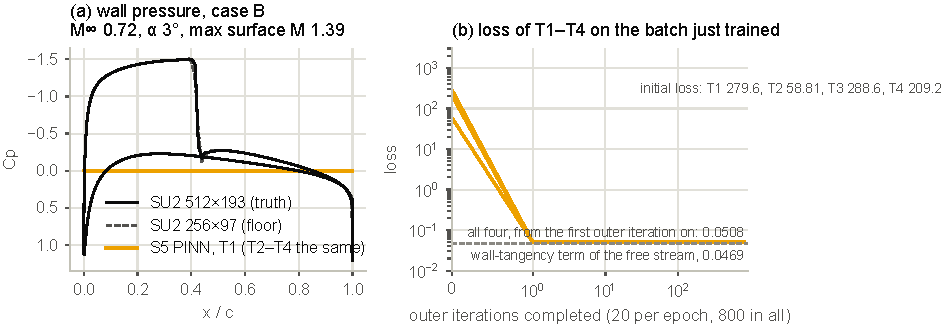
\includegraphics[width=\textwidth]{s5_gate.pdf}
\caption{The S5 gate on case B. (a) SU2's wall pressure, with the shock at $x\approx0.42$, and the
PINN's flat $\Cp = 0$. (b) The loss of T1--T4 after each outer iteration: one step from the initial
value to the uniform stream, then 800 outer iterations without change.}
\label{fig:s5gate}
\end{figure}

No configuration passes (\cref{tab:s5gate}, \cref{fig:s5gate}). Every one is in the uniform stream
found by the probe: it predicts $\CL\approx0$ against 0.574 and misses the shock. The gate took
2.53\,h in all, against its 72\,h budget. Each timed first epoch overestimated its run by 2.2--4.2
times, because a trapped run descends only in its first epoch.

Three readings of these numbers matter beyond the verdict.
\begin{itemize}
  \item \emph{A uniform stream scores only 5.2\,\% on the gate's metric.} RMAE divides by the
    field's range, and most of the box is near free stream. On step-3 case
    \texttt{test\_in-0004} the same metric gives the FNO 0.30\,\% at $256\times97$ and this
    study's potential PINN 1.23\,\%. So 1\,\% is a demanding threshold, not a loose one.
  \item \emph{The collapse flag misses this failure.} It asks whether the largest wall speed is
    below half the truth's, which catches fluid at rest. A uniform stream at $0.93\,U_\infty$ passes
    it. The gate's verdict does not use the flag.
  \item \emph{The closure cost varied twentyfold}, from 0.086\,s (T2) to 1.77\,s (T4), for runs in
    the same state. The cause was not identified.
\end{itemize}

\subsection{Predictions, and what S5 shows}
\label{sec:s5outcome}

\begin{table}[t]
\centering\small
\caption{The S5 predictions, recorded before any S5 code, and their outcomes.}
\label{tab:s5predictions}
\begin{tabularx}{\textwidth}{@{}>{\raggedright\arraybackslash}p{0.47\textwidth}>{\raggedright\arraybackslash}X@{}}
\toprule
Prediction & Outcome\\
\midrule
P4. The recipe passes the gate within T1--T4. & \textbf{Failed.} All four miss the 1\,\%
threshold by about five times, in the same uniform stream.\\
\addlinespace
P5. Reverting the residual weighting breaks R; reverting the encoding or the collocation does not;
R fails or collapses on the cylinder at $\Ma = 0.1$. & \textbf{Not tested}: with no R there is no
ablation.\\
\addlinespace
P6. In extrapolation the new PINN degrades less than the FNO, but stays above it in range. &
\textbf{Not tested}: no step-3 runs.\\
\addlinespace
P7. Per case, the new PINN still costs at least 10 times SU2's CPU time. & \textbf{Not tested}.\\
\bottomrule
\end{tabularx}
\end{table}

\paragraph{What S5 shows.}
Rebuilt from the paper on this study's grid, the recipe does not train. It falls into a uniform
stream from initialisation under all four tuning configurations. No single change probed keeps it
out of a trivial state: not the slope treatment, not the residual's weighting or balance, not the
optimiser, the embedding's scale or the initialisation, and not hard boundary conditions. Artificial
viscosity cannot help in such a state, because the viscous term is zero in each of them. This
study's first Euler PINN found fluid at rest; the rebuilt one finds a uniform stream. Both are the
same kind of failure: a minimum of the loss that satisfies the equations and violates only a soft
condition.

\paragraph{What it does not show.}
It does not show that the published result is wrong. Within S5 a flaw in the recipe cannot be told
apart from what the paper leaves unstated: the far-field distance of their PINN grid, how the
volume weights are normalised, the initialisation, the precision. Every probe and every gate run
used one seed. The probes ran three of the recipe's 800 outer iterations, except the one full
epoch. The uniform states are exact (a dead layer, outer iterations stalling in a few closures), so
they are traps in practice, not slow descents.

%===================================================================================================
\section{Discussion}
\label{sec:discussion}

\paragraph{The operator.}
The FNO does what operators promise: it learns the family well enough to beat a strong linear
baseline exactly where that baseline is weak, at moving shocks. But it reaches the floor only on
its own training grid and only in range. Its resolution transfer is $O(h)$, not exact: the padded
field jumps to zero at the wrap, and that jump aliases differently at each resolution. In
extrapolation its errors are biased in a way no in-range score would reveal. Economically it
repays its training only after about as many new cases as the campaign that trained it, as
predicted.

\paragraph{The PINN.}
The PINN's difficulties come from the formulation more than from the optimiser.
\begin{itemize}
  \item The Euler PINN, as configured here, has a degenerate minimiser: fluid at rest, which its
    soft far-field condition did not exclude.
  \item The full-potential PINN removes that minimiser and passes the cylinder warm-up. It still
    under-predicts the circulation on lifting sections, while the equal-speed Kutta term is met at
    the wrong circulation.
  \item The sharp trailing edge is the crux: there the map is degenerate, the corner flow is
    singular, and the condition that fixes the lift lives.
  \item Gradient-norm balancing, a standard remedy, made one run worse by handing the objective to
    the wall term.
\end{itemize}

\paragraph{A working transonic PINN in the literature.}
Wassing, Langer and Bekemeyer~\cite{wassing2025} solve the Euler equations, energy equation
included, for transonic NACA\,0012 flow with a PINN. Their method:
\begin{itemize}
  \item collocation at the points of a $400\times200$ elliptic O-grid, with Fourier features of
    the grid indices;
  \item soft far-field, wall and periodicity terms, and a volume-weighted residual scaled by
    $2\times10^4$;
  \item L-BFGS alone, in mini-batches;
  \item artificial viscosity localised by an analytic shock sensor times a stagnation-point
    sensor.
\end{itemize}
They report Cp errors of 0.3--0.4\,\% at $\Ma = 0.70$--$0.75$, and 3\,\% at 0.78. Without
viscosity, or with global viscosity and no sensors, they capture no shock. They impose no explicit
Kutta condition, yet their parametric network's lift agrees with the reference over
$\alpha\in(0,4)^\circ$ at $\Ma = 0.72$.
They train for 30--45\,min per case, against 5.6\,h for the \texttt{pure} runs here, on different
hardware.

Their result bounds this study's conclusions about PINNs. The collapse of the Euler PINN and the
low circulation of the potential PINN belong to the formulations and training tested here. Stage
S5 (\cref{sec:s5}) rebuilt their recipe on this study's grid to find out which of the many
differences matters. The rebuilt recipe did not train either: it fell into a uniform stream. The
question has moved rather than closed, and the list of differences now includes what their paper
leaves unstated. The global viscous variants specified in this study's
plan resemble their failing global form, though on a different formulation. They also conclude
that PINNs do not currently beat CFD for a single forward case, which agrees with P1.

\paragraph{Cost.}
A per-case PINN costs between 88 and 220 SU2 solutions, depending on how GPU and CPU time are
counted. At this problem size a forward-mode PINN is a learning exercise, not a solver; its
strengths lie in inverse problems and sparse data, which this study did not test.

\subsection{What the comparison does and does not show}
\label{sec:scope}

The results invite the conclusion that neural operators suit aerodynamics better than PINNs. The
study supports a narrower one. \emph{For many-query prediction inside a well-sampled design space,
when the CFD campaign can be paid for, a data-trained surrogate is the better tool, and a per-case
PINN is not competitive even with the CFD it would replace.} On that task the margin is wide:
\begin{itemize}
  \item in range, the FNO's near-field error is 1.3--5.3 times the floor, against 26--65 times for
    the PINN, whose lift is 64--101\,\% low on five of six cases (\cref{tab:results,tab:pinncl});
  \item a new case costs 0.054\,s with the FNO, against 5.6\,h with the PINN, which is 88--220 SU2
    runs (\cref{tab:costs}).
\end{itemize}

Five things keep this from being a general verdict on the two families.
\begin{enumerate}
  \item \textbf{The contestants answered different questions.} The FNO learned from 881 SU2
    solutions, about 64 CPU-hours of CFD. The PINN was given no data at all. A PINN solving one
    forward case that CFD already solves well is the PINN's least favourable use, which is why P1
    was predicted.
  \item \textbf{This study's PINN is not the state of the art.} The Euler PINN of Wassing, Langer and
    Bekemeyer~\cite{wassing2025} reaches 0.3--0.4\,\% Cp error on transonic NACA\,0012 cases, in
    30--45\,min per case, with no explicit Kutta condition. The accuracy of the PINN here says more
    about the formulations tried than about PINNs. Rebuilt from their paper on this study's grid,
    their recipe failed too (\cref{sec:s5}). The published result does not transfer from the paper
    alone, but nothing here shows it wrong. Even so, they reach the same conclusion on cost: a PINN
    does not currently beat CFD for a single forward case.
  \item \textbf{The operator's win is narrower than it looks.}
    \begin{itemize}
      \item It repays its training only after 1,126 new cases; for fewer, running SU2 is cheaper
        (\cref{fig:breakeven}).
      \item POD, a linear baseline, beats it on in-range subcritical cases at $256\times97$. The FNO
        clearly earns its complexity only on supercritical cases, where shocks move with the inputs.
      \item Outside the training range it fails: 3.6 times the floor, with drag errors up to 181
        counts, biased rather than scattered.
      \item Its shocks are smeared, and its subcritical near-field entropy falls below free stream on
        9--24 of 37 cases, which SU2's never does.
    \end{itemize}
  \item \textbf{This is the easy end of aerodynamics.} The problem is two-dimensional, steady and
    inviscid, one family of sections with four inputs, on one structured grid. Practical
    aerodynamics is three-dimensional, viscous and turbulent, over varied geometry. There each
    training solution costs hours, a thousand of them is a real expense, and an operator must
    generalise across shapes and meshes. None of that was tested.
  \item \textbf{The settings where PINNs are argued to be strong were not tested.} These are
    inverse problems, sparse measurements such as surface pressure taps, and parametric PINNs: one
    network trained across a range of inputs from the equations alone. The parametric network of
    Wassing et al.\ answers in 35\,ms after 1.5--2.75\,h of training. It amortises its cost the way
    an operator does, without needing a CFD campaign. Physics-informed neural operators, which add
    the equation residual to an operator's training, were left as an extension.
\end{enumerate}

Which approach suits a given aerodynamic task therefore depends on three questions that this study
answers for only one setting:
\begin{itemize}
  \item how many queries are needed (against the break-even of \cref{eq:breakeven});
  \item whether the queries stay inside the sampled range;
  \item whether training data can be afforded at all.
\end{itemize}
All the accuracy figures are also relative to SU2 at $512\times193$, which on the anchor case is
itself 6--8\,\% low in lift (\cref{tab:vj}). That leaves the ranking unchanged but limits any claim
about absolute accuracy.

\subsection{Limitations}
\begin{itemize}
  \item The costs mix hardware: SU2 and POD on the CPU, the FNO on the Apple GPU, and the PINN on
    both.
  \item The PINN results are single runs on three cases per regime.
  \item The POD selection sits on the edge of its search grid.
  \item The three SU2 grids are not in the asymptotic range, so the floor is a grid difference,
    not an extrapolated error. On the transonic anchor the truth itself is 6--8\,\% low in lift
    against a grid-converged reference (\cref{tab:vj}).
  \item The 100-chord outer boundary truncates $\CL$ at the $10^{-3}$ level, equally for every
    method.
  \item The PINN's learned $\Gamma$ was not recorded during training; it is inferred from the
    scored lift.
\end{itemize}

%===================================================================================================
\section{Open items and reproducibility}
\label{sec:repro}

\paragraph{Still open.}
\begin{itemize}
  \item Why Wassing, Langer and Bekemeyer's Euler PINN~\cite{wassing2025}, rebuilt from the paper,
    falls into a uniform stream on this study's grid (\cref{sec:s5}). The candidates left are what
    the paper does not state: the far-field distance of their PINN grid, how the volume weights
    are normalised, the initialisation and the precision. Also open: whether a localised
    viscosity would fix the potential PINN's circulation.
  \item Why this study's SU2 grids fall short of the grid-converged anchor values: section, far
    field, grid and scheme are not separated.
  \item The expansion-shock test and an FNO ringing metric were not made. S5's ablation and its
    extrapolation comparison did not run, because its gate failed.
\end{itemize}

\paragraph{Reproducing the work.}
Every stage is one resumable script, run from the repository root (\cref{tab:repro}). The
committed records under \texttt{results/} are what every number here is read from. The SU2 cases,
datasets and predictions (about 8\,GB) are not committed but can be regenerated with those scripts.
\Cref{fig:fields,fig:warmup,fig:showcase} read those regenerated files.

\begin{table}[h]
\centering\small
\caption{The stage commands (SU2 found through \texttt{SU2\_BIN\_DIR}).}
\label{tab:repro}
\begin{tabular}{@{}lll@{}}
\toprule
Stage & Command & Writes\\
\midrule
S0 & \cmd{python scripts/s0\_check.py} & \cmd{results/s0/}\\
S1 & \cmd{python scripts/s1\_campaign.py train} (then \cmd{fine}) & \cmd{runs/su2/}\\
 & \cmd{python scripts/build\_dataset.py} & \cmd{data/hdf5/}, \cmd{results/s1/}\\
S2 & \cmd{python scripts/s2\_operator.py tune | final | pod} & \cmd{runs/predictions/}, \cmd{results/s2/}\\
S3a & \cmd{python scripts/s3\_warmup.py} & \cmd{results/s3/warmup.json}\\
S3 & \cmd{python scripts/s3\_pinn.py --shard K/N} & \cmd{runs/predictions/}, \cmd{results/s3/}\\
S4 & \cmd{python scripts/s4\_score.py} & \cmd{results/s4/}\\
S5 & \cmd{python scripts/s5\_su2.py} & \cmd{runs/su2/}, \cmd{results/s5/su2.json}\\
 & \cmd{python scripts/s5\_pinn.py gate} & \cmd{results/s5/gate.json}\\
 & \cmd{python scripts/s5\_score.py} & \cmd{results/s5/}\\
 & \cmd{python scripts/probes/probe\_s5\_*.py} & \cmd{results/s5/probe\_*.log}\\
Figures & \cmd{python docs/report/make\_figures.py} & \cmd{docs/report/figures/}\\
\bottomrule
\end{tabular}
\end{table}

%===================================================================================================
\appendix
% Appendices of report.tex: the learned models explained in detail, for teaching.
% Included after \appendix. Every number is the implementation's (src/apno) or a measured record.

\section{Neural networks from the ground up}
\label{app:basics}

\Cref{app:basics,app:fno,app:pinn,app:compare} explain the learned models of this study in enough
detail to rebuild them. This appendix covers the building blocks they share.
\Cref{app:fno} covers the Fourier neural operator and \cref{app:pinn} the physics-informed network,
each exactly as implemented in \texttt{src/apno/models}. \Cref{app:compare} sets the three models
side by side. Throughout, $\bm\theta$ denotes all the trainable parameters of a model.

\subsection{A network is a parameterised function}

The simplest network, and the one the PINN uses, is the \emph{multilayer perceptron} (MLP). It
maps an input vector $\bm x\in\mathbb R^{n_0}$ to an output $\bm y$ by alternating affine maps with
a fixed nonlinear function $\sigma$, applied element by element:
\begin{equation}
  \bm h^{0} = \bm x,\qquad
  \bm h^{\ell} = \sigma\!\bigl(\bm W^{\ell}\bm h^{\ell-1} + \bm b^{\ell}\bigr)\quad(\ell = 1,\dots,L),\qquad
  \bm y = \bm W^{L+1}\bm h^{L} + \bm b^{L+1}.
  \label{eq:mlp}
\end{equation}
\begin{itemize}
  \item The weight matrices $\bm W^\ell\in\mathbb R^{n_\ell\times n_{\ell-1}}$ and bias vectors
    $\bm b^\ell$ are the parameters, $n_\ell n_{\ell-1} + n_\ell$ of them per layer.
  \item $L$ is the \emph{depth}; $n_\ell$ is the \emph{width} of layer $\ell$.
  \item The PINN's network maps 3 inputs through $L = 7$ hidden layers of 96 units to one output.
    It has $(3\cdot96+96) + 6\,(96\cdot96+96) + (96+1) = 56{,}353$ parameters, plus the
    circulation $\Gamma$.
\end{itemize}

\paragraph{Why the nonlinearity matters.}
Without $\sigma$, \cref{eq:mlp} collapses to a single affine map, however deep it is. With a
nonlinear $\sigma$, a wide enough network can approximate any continuous function on a bounded set
to any accuracy (the universal approximation property). It says nothing about how hard the right
parameters are to \emph{find}, which is the whole difficulty in practice.

\paragraph{Activation functions.}
\Cref{fig:activations} compares the three activation functions relevant here.
\begin{itemize}
  \item \emph{tanh} is smooth and bounded, and has non-zero derivatives of every order.
  \item \emph{GELU}, $z\,\Phi(z)$ with $\Phi$ the standard normal distribution function, is a
    smooth version of the ReLU.
  \item \emph{ReLU}, $\max(z, 0)$, is piecewise linear: its second derivative is zero everywhere
    except at $z = 0$.
\end{itemize}
The choice matters for a PINN. A ReLU network is piecewise linear in its inputs, so every second
derivative of its output is zero almost everywhere, yet the full-potential residual is built from
second derivatives of the potential. This is why PINNs use tanh. The FNO only needs function values,
not derivatives, so it uses GELU.

\paragraph{Initialisation.}
Training starts from random parameters. PyTorch draws each affine layer's weights and biases
uniformly from $(-1/\sqrt{n_{\ell-1}},\ 1/\sqrt{n_{\ell-1}})$, which keeps each layer's initial
outputs of moderate size whatever its width. Fixing the random seed makes a run repeatable.

\begin{figure}[t]
\centering
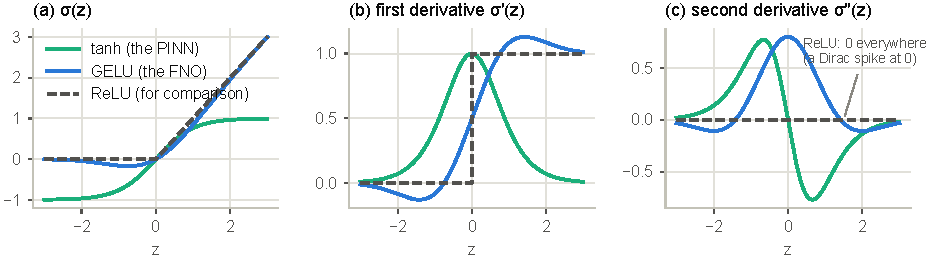
\includegraphics[width=\textwidth]{activations.pdf}
\caption{The activation functions used here and their derivatives. A PINN's loss contains
derivatives of the network with respect to its \emph{inputs}, so the activation's own derivatives
appear in the equations being solved. A ReLU network's second derivatives are zero almost
everywhere.}
\label{fig:activations}
\end{figure}

\subsection{Training is optimisation}

\paragraph{The loss.}
A \emph{loss} $\mathcal L(\bm\theta)$ is a single number that measures how wrong the network is.
\begin{itemize}
  \item In \emph{supervised} learning, as for the FNO, it compares the network's output with known
    answers: here, SU2's fields for the training cases.
  \item In \emph{physics-informed} learning, as for the PINN, there are no answers. The loss is how
    badly the network's output violates the governing equations and boundary conditions.
\end{itemize}
Training means finding parameters that make the loss small.

\paragraph{Gradient descent.}
The basic method steps against the gradient,
\begin{equation}
  \bm\theta \leftarrow \bm\theta - \eta\,\nabla_{\bm\theta}\mathcal L,
\end{equation}
with a \emph{learning rate} $\eta$.

\paragraph{Stochastic gradients.}
Computing the loss over all the data at every step is expensive, so the gradient is estimated
from a small random subset:
\begin{itemize}
  \item the FNO uses a \emph{mini-batch} of 8 cases per step, and one pass over all the training
    cases is an \emph{epoch};
  \item the PINN uses one set of 20,000 random collocation points, redrawn every 1,000 steps.
\end{itemize}
The noise in such estimates is tolerated, and it can even help an optimiser leave poor regions.

\subsection{Automatic differentiation}
\label{app:autodiff}

\paragraph{Reverse mode.}
Gradients are never derived by hand. PyTorch records every elementary operation of the forward
computation as a graph and then applies the chain rule backwards through it (\emph{reverse-mode
automatic differentiation}, or backpropagation). The gradient of a scalar loss with respect to all
parameters then costs a small multiple of one forward pass, however many parameters there are.

\paragraph{Derivatives with respect to the inputs.}
A PINN needs a second kind of derivative: of the network's \emph{output} with respect to its
\emph{inputs}, such as $\partial\psi/\partial\xi$. These come from the same machinery. In the code,
\begin{center}
\cmd{torch.autograd.grad(f.sum(), xi, create\_graph=True)}
\end{center}
returns $\partial f/\partial\xi$ at every collocation point at once. Summing first is legitimate
because each point's output depends only on that point's input, so the derivative of the sum with
respect to the $n$-th input is the derivative of the $n$-th output.

\paragraph{Differentiating a derivative.}
The flag \cmd{create\_graph=True} records the derivative computation itself as part of the graph,
so the derivative can be differentiated again. This nesting is what PINNs are built from:
\begin{itemize}
  \item the potential PINN differentiates $\psi$ once for the velocity;
  \item it differentiates again for the divergence in the residual;
  \item training then differentiates the loss with respect to $\bm\theta$ through both levels.
\end{itemize}
\Cref{app:pinnderivs} counts what that costs.

\subsection{Optimisers}

\paragraph{Adam.}
Adam~\cite{kingma2015adam} keeps running averages of the gradient $\bm g_t$ and of its element-wise
square, corrects their start-up bias, and scales each parameter's step by its own gradient history:
\begin{equation}
  \bm m_t = \beta_1\bm m_{t-1} + (1-\beta_1)\bm g_t,\quad
  \bm v_t = \beta_2\bm v_{t-1} + (1-\beta_2)\bm g_t^2,\quad
  \bm\theta_t = \bm\theta_{t-1} - \eta_t\,\frac{\bm m_t/(1-\beta_1^t)}{\sqrt{\bm v_t/(1-\beta_2^t)} + \epsilon},
  \label{eq:adam}
\end{equation}
with $\beta_1 = 0.9$, $\beta_2 = 0.999$ and $\epsilon = 10^{-8}$. Because every parameter gets its
own step size, Adam copes with losses whose sensitivity varies by orders of magnitude between
parameters. That is common in both networks here.

\paragraph{AdamW.}
AdamW~\cite{loshchilov2019adamw}, used for the FNO, adds \emph{decoupled} weight decay: it also
shrinks every weight by $\eta_t\lambda\bm\theta$ at each step ($\lambda = 10^{-4}$). This is
separate from the gradient, which discourages large weights without distorting Adam's scaling.

\paragraph{Learning-rate schedules.}
Large steps make fast early progress; small steps settle into a minimum. Both networks lower
$\eta_t$ as training proceeds:
\begin{equation}
  \text{FNO (cosine): }\ \eta_e = \tfrac12\eta_0\bigl(1 + \cos(\pi e/E)\bigr),\qquad
  \text{PINN (exponential): }\ \eta_k = \eta_0\,(\eta_1/\eta_0)^{k/K}.
\end{equation}
Here $e$ is the epoch of $E$ (300 in the final runs), $k$ the step of $K = 30{,}000$, and
$\eta_0 = 10^{-3}$, $\eta_1 = 10^{-4}$.

\paragraph{L-BFGS.}
L-BFGS~\cite{liu1989lbfgs} is a quasi-Newton method, used to finish the PINN's training. It builds
an approximation of the inverse Hessian from the last $m = 50$ pairs
\begin{equation}
  \bm s_k = \bm\theta_{k+1} - \bm\theta_k,\qquad \bm y_k = \nabla\mathcal L_{k+1} - \nabla\mathcal L_k,
\end{equation}
turns the gradient into a Newton-like search direction, and chooses the step length by a line
search satisfying the strong Wolfe conditions. Near a minimum it converges far faster than Adam.
It needs two things Adam does not:
\begin{itemize}
  \item \emph{A fixed objective.} If the collocation points changed between iterations, $\bm y_k$
    would mix a change in the function with a change in its sampling, and the line search would
    chase a moving target.
  \item \emph{Accurate arithmetic.} $\bm y_k$ is a difference of two nearly equal gradients, so in
    float32, with about 7 significant digits, it soon becomes mostly round-off. L-BFGS therefore
    runs in float64, on the CPU, because the Apple GPU has no float64.
\end{itemize}

\subsection{Generalisation, and what it means for each model}

A supervised model is judged on cases it never saw. The data are therefore split three ways:
\begin{itemize}
  \item a \emph{training set}, used to fit $\bm\theta$;
  \item a \emph{validation set}, used to choose hyperparameters and when to stop;
  \item a \emph{test set}, used once, for the final score.
\end{itemize}
\emph{Early stopping} keeps the parameters from the epoch with the lowest validation loss, and stops
when it has not improved for a set number of epochs (the \emph{patience}). Training several
\emph{seeds} (initialisations and batch orders) shows how much of a result is luck.

A PINN has no training set and nothing to generalise to: it fits one case. Its only test is the
comparison with SU2, which it never sees. The lesson of this study is that for a PINN a small loss
is not the same as a right answer (\cref{app:lessons}).

\subsection*{Questions}
\begin{enumerate}[label=Q\arabic*., leftmargin=*]
\item \textit{Why could a ReLU network not serve as the PINN here?}\newline
The full-potential residual contains second derivatives of the potential. A ReLU network is
piecewise linear, so its second derivatives vanish almost everywhere, and the residual would not
see the curvature that the equation constrains.
\item \textit{Why does the L-BFGS phase keep one fixed set of collocation points?}\newline
Its curvature pairs and its line search assume one deterministic function. Resampled points would
make every gradient difference partly sampling noise.
\item \textit{What does early stopping select, and from which data?}\newline
The epoch with the lowest validation loss. Test cases are never used for any choice.
\end{enumerate}

%---------------------------------------------------------------------------------------------------
\section{The Fourier neural operator in detail}
\label{app:fno}

\subsection{Learning an operator}

An ordinary network maps vectors to vectors. A \emph{neural operator} maps functions to functions.
Here the input function is the geometry and free stream, given as six fields over the grid, and the
output function is the flow state over the same grid:
\begin{equation}
\begin{aligned}
  \mathcal G:\quad \bm a(i,j) &= \bigl(\text{position},\ \text{ring index},\ \Ma,\ \cos\alpha,\ \sin\alpha\bigr)\\
  \longmapsto\quad \bm y(i,j) &= \text{the four targets of \cref{eq:targets}}.
\end{aligned}
\end{equation}
The operator is learned from 881 examples of the pair $(\bm a,\bm y)$. Ideally its parameters do
not depend on the grid, so a model trained at one resolution can be evaluated at another; the
measured resolution transfer error tests how far that holds here.

\subsection{From kernel integrals to Fourier multipliers}

A neural-operator layer replaces the matrix of an MLP by an integral operator acting on the hidden
function $\bm h(\bm z)$:
\begin{equation}
  \bm h_{\ell+1}(\bm z) = \sigma\!\left(\bm W\bm h_\ell(\bm z) + \int\kappa_{\bm\vartheta}(\bm z - \bm z')\,\bm h_\ell(\bm z')\,\mathrm d\bm z'\right).
\end{equation}
If the kernel $\kappa$ depends only on $\bm z - \bm z'$, the integral is a convolution. The
convolution theorem then turns it into a product in Fourier space,
\begin{equation}
  (\kappa * \bm h)(\bm z) = \mathcal F^{-1}\bigl[\hat\kappa(\bm k)\,\hat{\bm h}(\bm k)\bigr](\bm z).
\end{equation}
The FNO~\cite{li2021fno} learns $\hat\kappa$ directly: one complex $w\times w$ matrix
$\bm R_{\bm k}$ for each retained wavenumber $\bm k$, where $w$ is the number of hidden channels.
High wavenumbers are dropped. On a grid, $\mathcal F$ is the fast Fourier transform, so the layer
costs $O(N\log N)$ for $N$ nodes, and it couples every node to every other in a single layer.

\subsection{The Fourier layer as implemented}

The hidden state is a tensor $\bm h\in\mathbb R^{B\times w\times N_I\times(N_J+P)}$: batch,
channels, nodes around the airfoil, and nodes outward including the padding. One Fourier layer
(\cref{fig:fnoarch}, bottom) does five things.
\begin{enumerate}
  \item \emph{Transform}: $\hat{\bm h} = \mathrm{rfft2}(\bm h)$. This is a full FFT along $i$ and a
    real FFT along $j$, which keeps only the non-negative $j$-frequencies, since the negative ones
    are their complex conjugates.
  \item \emph{Truncate and mix}: keep $i$-frequencies $k_i\in\{0,\dots,23\}\cup\{-24,\dots,-1\}$
    and $j$-frequencies $k_j\in\{0,\dots,7\}$. At each kept mode, mix the channels with that mode's
    own complex matrix,
    \begin{equation}
      \hat o_{b,o,\bm k} = \sum_{c=1}^{w}\hat h_{b,c,\bm k}\,R_{c,o,\bm k},
    \end{equation}
    and set every other mode to zero. Positive and negative $k_i$ need separate weight tensors
    (\cmd{w\_pos} and \cmd{w\_neg}), because the real FFT halves only the $j$ axis.
  \item \emph{Inverse transform} back to the grid.
  \item \emph{Pointwise path}: add $\bm W\bm h + \bm b$, a $1\times1$ convolution, which mixes
    channels at each node with no spatial coupling.
  \item \emph{Activation}: apply GELU, except after the last layer.
\end{enumerate}

\paragraph{Why the pointwise path is needed.}
The spectral path can carry only $48\times8$ modes. The pointwise path passes everything else, the
fine detail that nonlinearities create in particular, and it is not tied to periodicity at all.
Without it, every layer's output would be a smooth, band-limited field.

\begin{figure}[t]
\centering
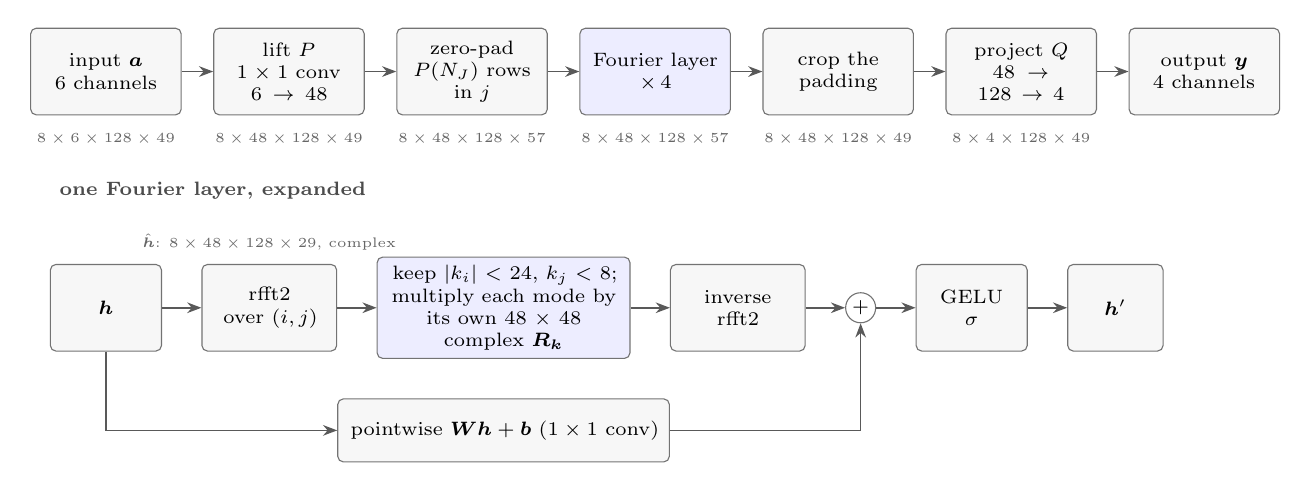
\begin{tikzpicture}[
  font=\scriptsize,
  blk/.style={draw=black!55, rounded corners=2pt, fill=black!3, align=center, inner sep=3pt,
              minimum height=11mm, text width=17mm},
  fl/.style={blk, fill=blue!7},
  arr/.style={-{Stealth[length=1.8mm]}, black!65, semithick},
  shp/.style={font=\tiny, text=black!60, align=center}]
\node[blk] (a) {input $\bm a$\\6 channels};
\node[blk, right=4mm of a] (P) {lift $P$\\$1\times1$ conv\\$6\to48$};
\node[blk, right=4mm of P] (pad) {zero-pad\\$P(N_J)$ rows\\in $j$};
\node[fl, right=4mm of pad] (F) {Fourier layer\\$\times\,4$};
\node[blk, right=4mm of F] (crop) {crop the\\padding};
\node[blk, right=4mm of crop] (Q) {project $Q$\\$48\to128\to4$};
\node[blk, right=4mm of Q] (y) {output $\bm y$\\4 channels};
\foreach \u/\v in {a/P, P/pad, pad/F, F/crop, crop/Q, Q/y} \draw[arr] (\u) -- (\v);
\node[shp, below=1mm of a] {$8\times6\times128\times49$};
\node[shp, below=1mm of P] {$8\times48\times128\times49$};
\node[shp, below=1mm of pad] {$8\times48\times128\times57$};
\node[shp, below=1mm of F] {$8\times48\times128\times57$};
\node[shp, below=1mm of crop] {$8\times48\times128\times49$};
\node[shp, below=1mm of Q] {$8\times4\times128\times49$};
% the Fourier layer, expanded
\begin{scope}[yshift=-30mm]
\node[blk, text width=12mm] (h) {$\bm h$};
\node[blk, right=5mm of h, text width=15mm] (fft) {rfft2\\over $(i,j)$};
\node[fl, right=5mm of fft, text width=30mm] (R) {keep $|k_i|<24$, $k_j<8$;\\multiply each mode by\\its own $48\times48$ complex $\bm R_{\bm k}$};
\node[blk, right=5mm of R, text width=15mm] (ifft) {inverse\\rfft2};
\node[circle, draw=black!55, right=5mm of ifft, inner sep=1pt] (plus) {$+$};
\node[blk, right=5mm of plus, text width=12mm] (act) {GELU\\$\sigma$};
\node[blk, below=5mm of R, text width=40mm, minimum height=8mm] (W) {pointwise $\bm W\bm h + \bm b$ ($1\times1$ conv)};
\node[blk, right=5mm of act, text width=10mm] (h2) {$\bm h'$};
\draw[arr] (h) -- (fft); \draw[arr] (fft) -- (R); \draw[arr] (R) -- (ifft); \draw[arr] (ifft) -- (plus);
\draw[arr] (plus) -- (act); \draw[arr] (act) -- (h2);
\draw[arr] (h.south) |- (W.west); \draw[arr] (W.east) -| (plus.south);
\node[shp, above=0.5mm of fft] {$\hat{\bm h}$: $8\times48\times128\times29$, complex};
\end{scope}
\node[font=\scriptsize\bfseries, black!70, anchor=south west] at ([yshift=7mm]h.north west) {one Fourier layer, expanded};
\end{tikzpicture}
\caption{The FNO as implemented, with tensor shapes (batch, channels, $i$, $j$) for a batch of 8 at
the $128\times49$ training resolution, with the selected width of 48. The projection is two
$1\times1$ convolutions with a GELU between them. At $256\times97$ the same
weights see $8\times48\times256\times113$ after padding, and the same $48\times8$ retained modes.
Bottom: one Fourier layer.}
\label{fig:fnoarch}
\end{figure}

\paragraph{Where the parameters are.}
\Cref{tab:fnoparams} counts the parameters. Almost all of them, 99.8\,\%, are spectral weights.
The model has about $7.1$ million real parameters, and the training set holds
$881\times4\times128\times49 = 22.1$ million target values. Weight decay, early stopping and
the truncation itself are what keep it from memorising them.

\begin{table}[t]
\centering\small
\caption{Parameters of the selected FNO (width 48, modes $24\times8$, 4 layers). A complex weight
counts as two real numbers.}
\label{tab:fnoparams}
\begin{tabular}{@{}lll r@{}}
\toprule
Part & Shape & Per part & Real numbers\\
\midrule
Lift $P$ & $48\times6$ weights $+\,48$ biases & & 336\\
Spectral weights $\bm R$, 4 layers & $2\times(48\times48\times24\times8)$ complex per layer & 1,769,472 & 7,077,888\\
Pointwise $\bm W$, 4 layers & $48\times48 + 48$ per layer & 2,352 & 9,408\\
Projection $Q$ & $(48\times128+128) + (128\times4+4)$ & & 6,788\\
\midrule
Total & & & 7,094,420\\
\bottomrule
\end{tabular}
\end{table}

\subsection{Working in the O-grid's index space}

\paragraph{Index space, not physical space.}
The FFT treats the grid as a uniform rectangle of nodes. The physical grid is curved and strongly
stretched: its first wall spacing is $2\times10^{-3}$ chords, while near the outer boundary the
spacing is chord-sized. A convolution in index space is translation-invariant in $(i,j)$, not in
$(x,y)$, so the geometry reaches the model only through the position channels. The model has to
learn what an index-space pattern means at each physical location.

\paragraph{Around the airfoil, periodicity is exact.}
Node $i = N_I$ is node $i = 0$, so the FFT along $i$ involves no approximation. Mode $k_i$ is
$k_i$ cycles per circuit of the airfoil at any $N_I$. This is what lets the same $\bm R_{\bm k}$
mean the same thing at $128$ and at $256$ nodes.

\paragraph{Outward, the field is not periodic.}
A plain FFT along $j$ would wrap the outer boundary onto the wall. Zero-padding by $P$ rows puts a
buffer between them:
\begin{equation}
  P = \tfrac{1}{6}(N_J - 1):\qquad
  \frac{48 + 8}{48} = \frac{96 + 16}{96} = \frac{7}{6},
\end{equation}
so the padded column spans the same $\eta$ at both resolutions. The discrete period in $\eta$ is
$(N_J + P)\,\Delta\eta = (N_J + P)/(N_J - 1)$, and it differs slightly: 57/48 against 113/96.
From 1 to 26 October the rule was $P = \mathrm{round}\bigl(\tfrac{3}{16}(N_J - 1)\bigr) - 1$ (8 and
17 rows), which makes the period $19/16$ at both, so that a learned radial mode means the same
physical frequency. On the trained networks 16 rows transferred better than 17, and the rule was
changed back (\cref{sec:fno}). The padded rows are zero only on entry. The layers write into them,
and they are cropped once, before the projection.

\paragraph{The transfer is still only first-order.}
At the end of the padding the field jumps back to the wall row's values, and that jump aliases
differently at the two resolutions. The measured transfer error is therefore not zero: on the
validation cases, the selected model's prediction at $128\times49$ differs from its prediction at
$256\times97$ by a relative L2 of 0.021 (0.035 with 17 rows). In the test scores this is the
factor of 1.7 between the two grids on in-range subcritical cases (\cref{tab:results}); with 17
rows it was 4.

\subsection{Inputs and outputs}

\paragraph{Inputs.}
The six input channels are given in \cref{sec:models}. The position channels are
$(x - \tfrac12,\ y)\,\ln(1+r)/r$. This keeps the direction of each node from mid-chord and
compresses its distance logarithmically: the outer circle at $r = 100$ maps to radius
$\ln101\approx4.6$, while the section is barely distorted. Without the compression, the far field
would dominate the coordinate values and the near-body detail would occupy a sliver of their range.

\paragraph{Outputs.}
The targets (\cref{eq:targets}) are each standardised per channel, over all training cases and
nodes: $z = (y - \mu_c)/s_c$. The network predicts $z$. A prediction is mapped back by inverting
the standardisation and then \cref{eq:targets}:
\begin{equation}
  \hat u = y_1 + \cos\alpha,\quad \hat v = y_2 + \sin\alpha,\quad
  \hat p = 1 + \tfrac12\gamma\Ma^2 y_3,\quad \hat\rho = 1 + \tfrac12\Ma^2 y_4.
\end{equation}

\subsection{Training}

\Cref{alg:fno} is the training loop as run. At $n = 896$ the training set is the 881 converged
cases among the first 896 Sobol points. An epoch is 111 mini-batches of 8, so 300 epochs are
33,300 AdamW steps, which took 36 minutes on the Apple GPU.

\Cref{fig:learning} shows the validation loss for each training-set size. Every curve still
improves at epoch 300: the best epochs are 274--297. The noise on each curve is the mini-batch
noise, filtered by the decaying learning rate. More data lowers the whole curve, but by less at
each doubling (\cref{tab:efficiency}).

\begin{algorithm}[t]
\caption{FNO training (\texttt{apno.models.train\_fno.train})}
\label{alg:fno}
\small
\begin{algorithmic}[1]
\Require training cases (the first $n$ Sobol points that converged), validation cases, seed
\State fit the per-channel standardiser on the training targets
\State $\bm X,\bm Z\gets$ features and standardised targets at every second node ($128\times49$)
\State initialise $\bm\theta$ from the seed; $v^\ast\gets\infty$
\For{epoch $e = 0,\dots,E-1$}
  \For{each mini-batch $b$ of 8 cases, in a fresh random order}
    \State $\mathcal L\gets\mathcal L_A$ (or $\mathcal L_B$) of $\mathrm{FNO}_{\bm\theta}(\bm X_b)$ against $\bm Z_b$
    \State $\bm\theta\gets\mathrm{AdamW}(\bm\theta,\nabla_{\bm\theta}\mathcal L)$
  \EndFor
  \State lower the learning rate (cosine); $v\gets$ validation loss
  \If{$v < v^\ast$} \State save $\bm\theta$ as the checkpoint; $v^\ast\gets v$; $e^\ast\gets e$
  \ElsIf{$e - e^\ast\ge30$} \State \textbf{stop}
  \EndIf
\EndFor
\State \Return the checkpoint (the epoch of lowest validation loss)
\end{algorithmic}
\end{algorithm}

\begin{figure}[t]
\centering
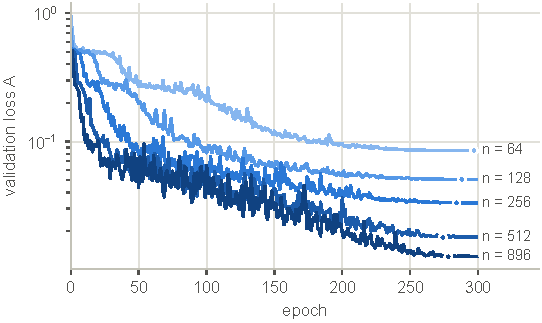
\includegraphics[width=0.66\textwidth]{learning_curves.pdf}
\caption{FNO validation loss per epoch for each training-set size $n$ (seed 0, loss A), darker
for larger $n$. Dots mark the epoch each run kept.}
\label{fig:learning}
\end{figure}

\subsection{What truncation does to a shock}

A truncated Fourier series of a function with a jump overshoots near the jump and oscillates on
both sides: the Gibbs phenomenon, an overshoot of about 9\,\% of the jump that does not shrink as
modes are added. \Cref{fig:truncation} applies the FNO's mode budget directly to the wall pressure
of the strongest showcase shock: the 24 lowest $i$-modes of each sign, out of 64, on the 128-node
training wall. The shock becomes a ramp with ripples on both sides.

The FNO is not a single filter. The pointwise paths and the nonlinearities generate the higher
frequencies that a filter alone would discard, so its own shocks are sharper than
\cref{fig:truncation}(a). The bias remains visible in the scores, though: its in-range shock
overshoot has median 0.42, against the floor's 0.19 (\cref{tab:shocks}).

\begin{figure}[t]
\centering
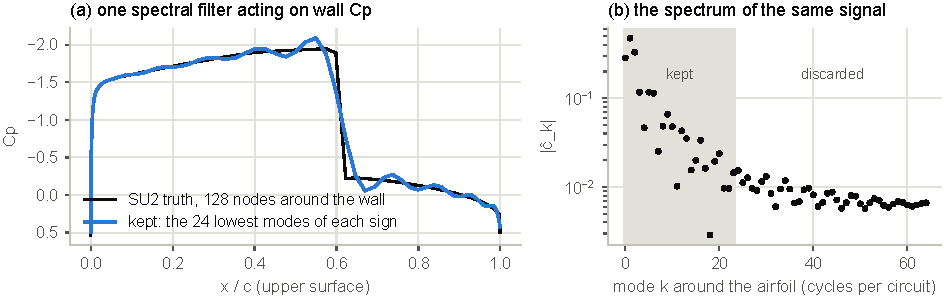
\includegraphics[width=\textwidth]{spectral_truncation.pdf}
\caption{(a) Wall $\Cp$ on the upper surface of \texttt{test\_in-0040} (SU2 truth at the
$128\times49$ training resolution), and the same signal keeping only the FNO's 24 lowest
$i$-modes of each sign. (b) The signal's Fourier amplitudes around the full wall. A shock puts
energy into every mode, and a slowly decaying tail is what a jump looks like in a spectrum.}
\label{fig:truncation}
\end{figure}

\subsection{Evaluation, and keeping the test set out}

\paragraph{Prediction.}
A prediction computes the six features on the case's own $256\times97$ grid, runs the network,
and inverts the target mapping. It takes 0.054\,s per case, about $4000$ times faster than an SU2
run.

\paragraph{Leakage guard.}
The data loader refuses to read a test split. Test inputs are read through a separate function that
returns only coordinates and free-stream values, never fields. A test case therefore cannot enter
training, normalisation or model selection by accident.

\subsection*{Questions}
\begin{enumerate}[label=Q\arabic*., leftmargin=*]
\item \textit{Why does a learned mode along $i$ mean the same thing at 128 and 256 nodes, while the $j$
direction needed a padding rule?}\newline
Along $i$ the grid is periodic with a period of one circuit at any $N_I$. Along $j$ the field is
not periodic, so it is padded; the period is then set by the $N_J + P$ padded samples and depends
on the choice of $P$. Matching the period exactly turned out to transfer worse on the trained
networks than matching the padded span.
\item \textit{How many complex weights does one Fourier layer hold, and why two tensors?}\newline
$2\times48\times48\times24\times8 = 884{,}736$. The real FFT halves only the $j$ axis, so positive
and negative $i$-frequencies are distinct modes, each with its own weights.
\item \textit{What was loss B meant to fix, and what happened?}\newline
Forces depend only on wall pressure, while a field loss is dominated by the many off-wall nodes.
Loss B adds the wall row with weight 10. In practice it was worse almost everywhere, and stopped
early at epoch 81 (\cref{sec:results}).
\item \textit{Why is the FNO's in-range subcritical error 1.7 times smaller on its training grid?}\newline
The resolution transfer is only first-order, because of the padding wrap; the same weights see
differently aliased fields at $256\times97$.
\end{enumerate}

%---------------------------------------------------------------------------------------------------
\section{The physics-informed neural network in detail}
\label{app:pinn}

\subsection{The idea}

A PINN~\cite{raissi2019pinn} represents the solution of \emph{one} problem as a network: a function
of continuous coordinates. It is trained so that the governing equations and boundary conditions
hold at many sampled points.
\begin{itemize}
  \item There is no training data. The equations supply the supervision, so the method can in
    principle solve a case nobody has solved.
  \item Derivatives are exact, by automatic differentiation, and there is no mesh to generate.
  \item The answer can be evaluated anywhere, at any resolution.
\end{itemize}
The price is that every new case is a fresh, non-convex optimisation, and its loss is a residual,
not an error.

\subsection{The network and its inputs}

The network is the MLP of \cref{eq:mlp} with 7 hidden layers of 96 tanh units. Its three inputs are
$(\cos2\pi\xi,\ \sin2\pi\xi,\ \eta)$, not $(x,y)$ and not $(\xi,\eta)$. Because $\xi$ enters only
through $\cos2\pi\xi$ and $\sin2\pi\xi$, the output satisfies $\psi(\xi + 1,\eta) = \psi(\xi,\eta)$
exactly: periodicity around the airfoil is built in, not learned. The full-potential network
outputs one scalar $\psi$ and has one more parameter, $\Gamma$, for 56,354 in all. The Euler network
outputs three, $(\ln\hat\rho,\ \hat u - \cos\alpha,\ \hat v - \sin\alpha)$, and has 56,547.

\paragraph{Why the circulation needs its own parameter.}
Around a lifting airfoil the potential is multivalued: one circuit around the body adds $\Gamma$ to
$\phi$. A network of $(\cos2\pi\xi, \sin2\pi\xi, \eta)$ is single-valued and cannot represent that
jump. The term $\Gamma\Theta_v$ carries it instead: $\Theta_v$ jumps by exactly one across the wake
cut, and its gradient, the velocity, is continuous there. The network therefore represents only
the single-valued remainder.

\subsection{Hard and soft constraints}

Every condition the solution must meet is either built into the representation (\emph{hard}),
holding for any $\bm\theta$, or added to the loss (\emph{soft}), holding only as well as the
optimiser manages. \Cref{tab:constraints} lists both formulations.

Each hard constraint removes a way to fail. Each soft one is something the optimiser may trade
against the others. The Euler PINN's failure here is this distinction at work: its far field was
soft, and the optimiser traded it away for fluid at rest. The full-potential PINN makes the far
field hard and puts the wall in the loss instead. A soft far field is not fatal in itself, though:
Wassing, Langer and Bekemeyer~\cite{wassing2025} keep it soft, weight the residual
$2\times10^4$ times more heavily, and succeed.

\begin{table}[t]
\centering\small
\caption{How each condition enters the two PINN formulations.}
\label{tab:constraints}
\begin{tabularx}{\textwidth}{@{}>{\raggedright\arraybackslash}p{0.2\textwidth}>{\raggedright\arraybackslash}X>{\raggedright\arraybackslash}X@{}}
\toprule
Condition & Euler PINN & Full-potential PINN\\
\midrule
Periodic around the airfoil & hard: inputs $\cos2\pi\xi$, $\sin2\pi\xi$ & hard: the same\\
Far field & soft: $(\hat\rho-1)^2 + |\hat{\vu} - \hat{\vu}_\infty|^2$ on 1,000 outer points, weight 10 & hard: $\psi(1-\eta) = 0$ on $\eta = 1$\\
Wall tangency & hard: normal component removed with weight $(1-\eta)^4$ & soft: $(\vu\cdot\hat{\bm n}_w)^2$ at 512 wall points, weight 10\\
Positive density & hard: $\hat\rho = \exp(\cdot)$ & hard: Bernoulli, base floored at $10^{-6}$\\
Constant total enthalpy & hard: pressure from $H_\infty$ & hard: Bernoulli at $H_\infty$\\
Irrotational, isentropic & not imposed & hard: $\vu = \nabla\phi$, $\hat p = \hat\rho^{\,\gamma}$\\
Momentum & residual (two equations) & identity\\
Continuity & residual & residual (the only equation)\\
Kutta condition & soft: $|\vu|^2 = 0$ at the trailing edge, weight 10 & soft: equal speeds at $\xi = \delta, 1-\delta$, weight 10\\
Circulation & implied by the velocity field & explicit parameter $\Gamma$\\
\bottomrule
\end{tabularx}
\end{table}

\subsection{Derivatives through the grid map}
\label{app:pinnderivs}

\paragraph{The chain rule through the map.}
The network is a function of $(\xi,\eta)$, but the equations are written in $(x,y)$. The map
\cref{eq:ogrid} links them, and its derivatives (the \emph{metric terms}) come from automatic
differentiation of the same function the mesh generator uses. By the chain rule,
\begin{equation}
  \begin{pmatrix}\phi_x\\ \phi_y\end{pmatrix}
  = \frac1J\begin{pmatrix} y_\eta & -y_\xi\\ -x_\eta & x_\xi\end{pmatrix}
    \begin{pmatrix}\phi_\xi\\ \phi_\eta\end{pmatrix},\qquad J = x_\xi y_\eta - x_\eta y_\xi .
\end{equation}

\paragraph{The divergence.}
The divergence of the mass flux $(f,g) = \rho(u,v)$ uses the strong conservation form
\cref{eq:strongform}. It is the same quantity, rearranged so that the metric terms sit inside the
derivatives, as in a finite-volume scheme. The test suite checks that uniform flow gives zero to
round-off through this operator on the curved grid.

\paragraph{The trailing edge.}
At the trailing-edge wall point $J = 0$, because $x_\xi = y_\xi = 0$ there. The velocity there is
$0/0$, and the code reports the Kutta stagnation value, zero, at that single point.

\paragraph{The cost of the derivatives.}
For one training step of the full-potential PINN, the derivatives nest as follows:
\begin{enumerate}
  \item a forward pass gives $\psi$ and hence $\phi$ at 20,000 points;
  \item a first differentiation gives $\phi_\xi$ and $\phi_\eta$, hence $u$, $v$, $\rho$ and
    $(f,g)$;
  \item a second differentiation, of $y_\eta f - x_\eta g$ with respect to $\xi$ and of
    $-y_\xi f + x_\xi g$ with respect to $\eta$, gives the residual $\mathcal R$, which involves
    second derivatives of $\psi$;
  \item backpropagation of the loss to $\bm\theta$ differentiates that whole graph once more.
\end{enumerate}
In effect the step computes third-order derivatives of the network. The Euler PINN's residual
needs only first derivatives of its outputs, because its fluxes are algebraic in the state. That is
why one full-potential Adam step cost 0.88\,s on the CPU against the Euler PINN's 0.60\,s, and
0.19\,s on the Apple GPU. \Cref{fig:pinngraph} draws the computation.

\begin{figure}[t]
\centering
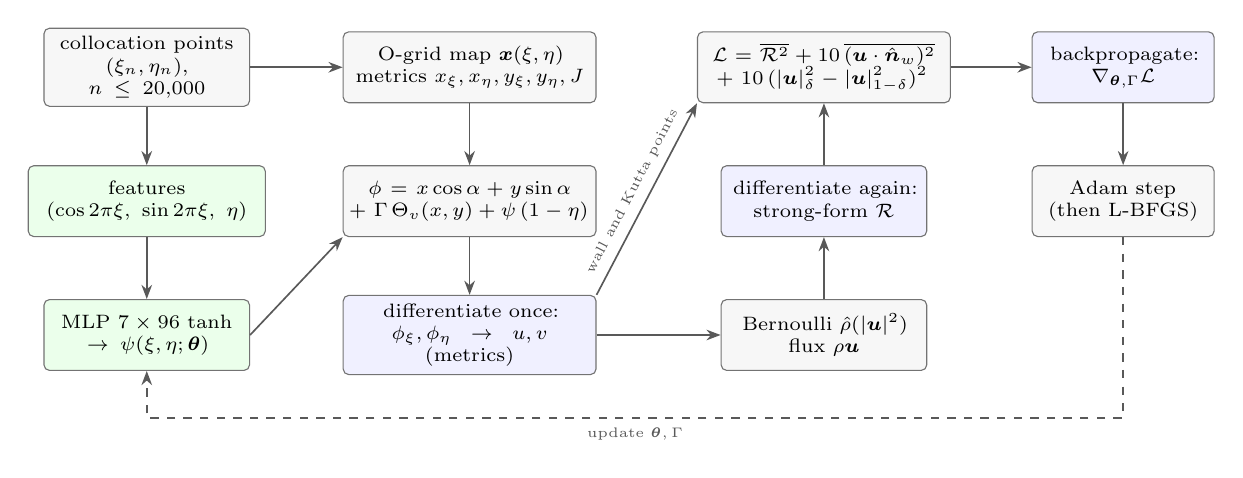
\begin{tikzpicture}[
  font=\scriptsize,
  blk/.style={draw=black!55, rounded corners=2pt, fill=black!3, align=center, inner sep=3pt,
              minimum height=9mm, text width=24mm},
  net/.style={blk, fill=green!8},
  ad/.style={blk, fill=blue!6},
  arr/.style={-{Stealth[length=1.8mm]}, black!65, semithick}]
\node[blk] (pts) at (0,0) {collocation points\\$(\xi_n,\eta_n)$, $n\le20{,}000$};
\node[net, text width=28mm] (feat) at (0,-1.7) {features\\$(\cos2\pi\xi,\ \sin2\pi\xi,\ \eta)$};
\node[net] (mlp) at (0,-3.4) {MLP $7\times96$ tanh\\$\to\psi(\xi,\eta;\bm\theta)$};
\node[blk, text width=30mm] (map) at (4.1,0) {O-grid map $\bm x(\xi,\eta)$\\metrics $x_\xi, x_\eta, y_\xi, y_\eta, J$};
\node[blk, text width=30mm] (phi) at (4.1,-1.7) {$\phi = x\cos\alpha + y\sin\alpha$\\$+\ \Gamma\,\Theta_v(x,y) + \psi\,(1-\eta)$};
\node[ad, text width=30mm] (vel) at (4.1,-3.4) {differentiate once:\\$\phi_\xi,\phi_\eta\ \to\ u, v$ (metrics)};
\node[blk, text width=30mm] (loss) at (8.6,0) {$\mathcal L = \overline{\mathcal R^2} + 10\,\overline{(\vu\cdot\hat{\bm n}_w)^2}$\\$+\ 10\,(|\vu|^2_\delta - |\vu|^2_{1-\delta})^2$};
\node[ad] (res) at (8.6,-1.7) {differentiate again:\\strong-form $\mathcal R$};
\node[blk] (rho) at (8.6,-3.4) {Bernoulli $\hat\rho(|\vu|^2)$\\flux $\rho\vu$};
\node[ad, text width=21mm] (bp) at (12.4,0) {backpropagate:\\$\nabla_{\bm\theta,\Gamma}\mathcal L$};
\node[blk, text width=21mm] (opt) at (12.4,-1.7) {Adam step\\(then L-BFGS)};
\draw[arr] (pts) -- (feat); \draw[arr] (feat) -- (mlp); \draw[arr] (pts) -- (map);
\draw[arr] (map) -- (phi); \draw[arr] (mlp.east) -- (phi.south west); \draw[arr] (phi) -- (vel);
\draw[arr] (vel) -- (rho); \draw[arr] (rho) -- (res); \draw[arr] (res) -- (loss);
\draw[arr] (vel.north east) -- node[sloped, above, font=\tiny, black!65] {wall and Kutta points} (loss.south west);
\draw[arr] (loss) -- (bp); \draw[arr] (bp) -- (opt);
\draw[arr, dashed] (opt.south) |- ([yshift=-6mm]mlp.south) node[pos=0.75, below, font=\tiny, black!65] {update $\bm\theta,\Gamma$} -- (mlp.south);
\end{tikzpicture}
\caption{One training step of the full-potential PINN. Green: the network. Blue: automatic
differentiation. The residual needs two nested derivatives of the network with respect to its
inputs, and the update differentiates through both.}
\label{fig:pinngraph}
\end{figure}

\subsection{Collocation points}

\paragraph{Where the points fall.}
Each draw is 20,000 points uniform in $(\xi,\eta)$, which the map turns into points strongly
clustered at the body (\cref{fig:collocation}). In the first draw of the production run on
\texttt{test\_in-0022}, 11,018 points lie within 2.5 chords of mid-chord, a disk that is 0.06\,\%
of the domain's area. Two consequences follow:
\begin{itemize}
  \item A mean over these points weights each physical region by $1/J$. That favours the near field
    where the answer matters, but it also means the loss barely sees most of the domain.
  \item Points are redrawn every 1,000 Adam steps, so the network cannot satisfy the equation only
    at a fixed set of points and be wrong between them.
\end{itemize}

\paragraph{The trailing-edge exclusion.}
After each draw, the points within 0.02 chord of the trailing edge are dropped (225 in the draw
shown). The corner flow is singular there, and those few points would otherwise dominate the
loss.

\paragraph{Wall points.}
The 512 wall points sit at $\xi = (k + \tfrac12)/512$, half a spacing off the grid, so that none
falls on the degenerate trailing-edge point.

\begin{figure}[t]
\centering
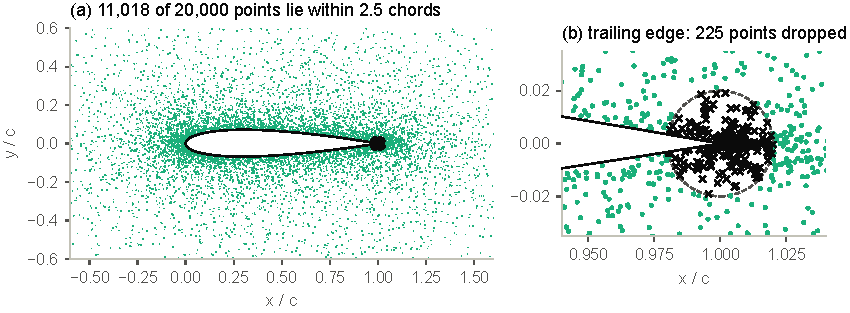
\includegraphics[width=\textwidth]{collocation.pdf}
\caption{The first draw of collocation points of the \texttt{pure} run on \texttt{test\_in-0022}
(seed 0, as drawn in production). Points uniform in $(\xi,\eta)$ crowd the section and its wake
line. Crosses: points inside the 0.02-chord trailing-edge exclusion (dashed circle), which are
dropped from the residual.}
\label{fig:collocation}
\end{figure}

\subsection{The loss and its weights}

\paragraph{One trade-off for several conditions.}
The loss \cref{eq:pinnloss} adds terms with different units and very different sizes and
sensitivities. Minimising a weighted sum finds one point on a trade-off between them. Only if the
network could satisfy every term exactly at once would the weights not matter, and with finite
networks and a singular corner it cannot. With fixed weights of 10, the \texttt{pure} runs ended
with residual $1$--$24\times10^{-3}$, wall term $0.5$--$21\times10^{-4}$ and Kutta term below
$6\times10^{-6}$ (\cref{tab:pinnruns}).

\paragraph{Gradient-norm balancing.}
Gradient-norm balancing~\cite{wang2021gradient} sets each weight from how strongly its term
pulls on the parameters, compared with the residual. It updates the weights by
\cref{eq:gradnorm} every 100 steps, which raises the weight of any term whose gradient is small.
The \texttt{gradnorm} run shows the risk. A term whose gradient is small \emph{because it is
already nearly satisfied} gets a huge weight: the Kutta weight reached $7\times10^{10}$. A term
that stays stubbornly unsatisfied, the wall term here, then holds most of the objective, and
L-BFGS spent its iterations on it at the residual's expense (\cref{fig:pinnhistory}).

\subsection{Optimisation}

\Cref{alg:pinn} is the training procedure. The two phases play to each optimiser's strength:
\begin{itemize}
  \item \emph{Adam}, robust to noisy, poorly scaled gradients, makes the large early progress in
    float32 on the GPU, over fresh points every 1,000 steps;
  \item \emph{L-BFGS} then converges locally on a fixed, deterministic objective in float64 on the
    CPU.
\end{itemize}
On the six \texttt{pure} runs the phases took similar time, 9,658\,s of Adam and 10,544\,s of
L-BFGS on average. Finally the network is evaluated at the $256\times97$ grid nodes in float64, and
the state is converted to the dataset's units, $p/p_\infty = \gamma\Ma^2\,p/(\rho_\infty U_\infty^2)$.

\begin{algorithm}[t]
\caption{PINN training for one case (\texttt{apno.models.train\_pinn.train})}
\label{alg:pinn}
\small
\begin{algorithmic}[1]
\Require the case $(\Ma,\alpha,t,m)$ and its O-grid map; no flow data
\State initialise $\bm\theta$ from seed 0; $\Gamma\gets0$; weights $w_{\mathrm{wall}} = w_K = 10$
\For{$k = 0,\dots,29{,}999$} \Comment{Adam, float32, Apple GPU}
  \If{$k \bmod 1000 = 0$}
    \State draw 20,000 points uniform in $(\xi,\eta)$; drop those within 0.02 chord of the trailing edge
  \EndIf
  \State evaluate $\mathcal R$, the wall term and the Kutta term; form $\mathcal L$ by \cref{eq:pinnloss}
  \If{gradient-norm balancing \textbf{and} $k \bmod 100 = 0$} \State update $w_{\mathrm{wall}}, w_K$ by \cref{eq:gradnorm}
  \EndIf
  \State $(\bm\theta,\Gamma)\gets\mathrm{Adam}\bigl((\bm\theta,\Gamma),\nabla\mathcal L\bigr)$; decay the learning rate exponentially
\EndFor
\State move the network and the last point set to the CPU in float64
\State run L-BFGS on that fixed objective: up to 5,000 iterations, history 50, strong Wolfe line search
\State \Return the network evaluated at the $256\times97$ nodes
\end{algorithmic}
\end{algorithm}

\subsection{Adaptive activations, and how a layer dies}
\label{app:deadlayer}

The S5 network (\cref{sec:s5recipe}) uses layer-wise adaptive activations~\cite{jagtap2020}:
\begin{equation}
  \sigma_k(x) = \tanh(n\,\omega_k x),\qquad
  \frac{\partial\sigma_k}{\partial x} = n\omega_k\,\mathrm{sech}^2(n\omega_k x),\qquad
  \frac{\partial\sigma_k}{\partial \omega_k} = n x\,\mathrm{sech}^2(n\omega_k x).
  \label{eq:adaptivetanh}
\end{equation}
One trainable number per layer sets how steep that layer's activation is. A steeper layer resolves
finer detail, and letting the optimiser choose the steepness speeds up early training.

The same freedom opens a trap. Suppose one slope reaches $\omega_k = 0$.
\begin{itemize}
  \item The layer's output is $\tanh(0) = 0$ for every input, so the layers after it see only their
    biases, and the network's output is a constant: a uniform field.
  \item The gradient with respect to every weight before layer $k$ passes through
    $\partial\sigma_k/\partial x = 0$, so it vanishes. Those weights receive no signal.
  \item Only $\omega_k$ itself still has a gradient, $\partial\sigma_k/\partial\omega_k = n z_k$,
    where $z_k(\bm r)$ is the layer's pre-activation. Reviving the layer therefore changes the
    field along one fixed function, set by the dead layer's weights.
\end{itemize}
In S5 that function is random and varies from cell to cell (\cref{eq:fourierfeatures}). Any step
along it adds far more residual than it removes wall-tangency error, so the best step is almost
zero, and the layer stays dead.

Jagtap et al.\ add a \emph{slope-recovery} term to the loss, $S = 1/\bigl(\tfrac1K\sum_k
e^{\omega_k}\bigr)$, which falls as the slopes grow. Because it averages over the layers, it can be
satisfied by steepening the live layers while one stays dead. That is what the S5 probe measured:
slopes of $n\omega$ up to 108 beside a zero (\cref{tab:s5probes}). A per-layer floor on $|\omega_k|$
would close that loophole. The probes suggest it would not be enough, though. With the slopes
frozen, the network found other trivial states, a vacuum and fluid at rest.

\subsection{What this study teaches about PINNs}
\label{app:lessons}

\begin{enumerate}
  \item \textbf{The formulation decides whether the minimum is the answer.} The Euler PINN's loss
    had a better minimum than the true flow: fluid at rest near the body, reaching the free stream
    only at the outer circle. Here, changing the equations and the hard constraints fixed that.
    Wassing, Langer and Bekemeyer~\cite{wassing2025} reach a working Euler PINN by other means,
    with different weighting, inputs and optimiser, so the minimum is a property of the whole
    formulation, loss weights included, not of the Euler equations alone. Rebuilt here from their
    paper (\cref{sec:s5}), their recipe found another such minimum, a uniform stream.
  \item \textbf{Geometric singularities dominate.} At a sharp trailing edge the map is degenerate
    and the true flow is singular. Before the fixes, ten of 20,000 points carried 99.9\,\% of the
    initial residual.
  \item \textbf{A small loss is not a right answer.} Every \texttt{pure} run ended with a residual
    of $10^{-3}$ to $2\times10^{-2}$ and a Kutta term met to $6\times10^{-6}$ or better, and five of the six had lift
    far too low. Without the Kutta term the loss was lower still (\cref{fig:pinnhistory}(a)):
    without it every circulation gives an admissible potential flow, so the loss cannot tell them
    apart. Only a comparison with an independent solution exposes this.
  \item \textbf{Automatic weighting is not automatically better.} Balancing by gradient norms
    handed the objective to the hardest term and wrecked the equation residual.
  \item \textbf{Each case costs a full training.} The 56,354 parameters are refitted from scratch
    with third-order automatic differentiation on 20,000 points for 30,000 Adam steps and up to
    5,000 L-BFGS iterations: about 5.6 hours here, against 3.5 minutes for SU2.
  \item \textbf{Trivial states are the default, not the exception.} A uniform stream, fluid at
    rest and a vacuum all satisfy the Euler equations. A soft boundary condition is all that
    separates them from the answer. In S5 every single change tried fell into one of them, or into
    a low-density state when both conditions were made exact (\cref{tab:s5probes}). Its
    artificial viscosity never acted, because the viscous term is zero in a trivial state.
\end{enumerate}

\subsection*{Questions}
\begin{enumerate}[label=Q\arabic*., leftmargin=*]
\item \textit{Which conditions are exact in the full-potential PINN, and which are penalties?}\newline
Periodicity, the far field, positive density, constant total enthalpy, irrotationality and
isentropy are exact. Continuity, wall tangency and the Kutta condition are in the loss
(\cref{tab:constraints}).
\item \textit{Why does a single-valued network need the extra term $\Gamma\Theta_v$?}\newline
A lifting flow's potential jumps by $\Gamma$ around the body. The network's inputs make it
single-valued, so the jump must be supplied by a term that carries it, with a continuous gradient.
\item \textit{Why is a full-potential Adam step dearer than an Euler one?}\newline
Its residual already contains second derivatives of the network, so backpropagation works through
third-order terms. The Euler residual needs only first derivatives.
\item \textit{The \texttt{nokutta} run reached a lower loss than \texttt{pure}. Why is it not better?}\newline
Without the Kutta term the problem has a family of solutions, one per circulation, and all of them
satisfy the remaining terms equally well. The loss cannot select the physical one, and neither run
found it.
\item \textit{In S5 the gradient with respect to a dead layer's slope is not zero. Why does
L-BFGS not revive the layer?}\newline
It can move the slope, but only along one fixed, cell-scale function: the dead layer's
pre-activation (\cref{app:deadlayer}). Along that function the weighted residual's curvature is
huge, and the wall term's gain is small. The minimum along the line lies almost at zero slope, and
the line search finds no decrease worth taking. The outer iterations stall in a few evaluations.
\end{enumerate}

%---------------------------------------------------------------------------------------------------
\section{The three models side by side}
\label{app:compare}

\begin{table}[h]
\centering\small
\caption{The learned models compared, with this study's figures.}
\label{tab:compare}
\begin{tabularx}{\textwidth}{@{}>{\raggedright\arraybackslash}p{0.17\textwidth}>{\raggedright\arraybackslash}X>{\raggedright\arraybackslash}X>{\raggedright\arraybackslash}X@{}}
\toprule
& FNO & POD + RBF & PINN (full potential)\\
\midrule
What it learns & an operator: inputs $\mapsto$ fields, for the whole family & a linear subspace of fields, and smooth weights over the inputs & one solution, as a continuous function\\
Data needed & 881 SU2 solutions & 881 SU2 solutions & none: the equations\\
Fitted parameters & 7.09\,M real, by AdamW & 256 modes of 99,328 values ($25$\,M numbers) plus RBF weights, by linear algebra & 56,354, by Adam then L-BFGS\\
One-off cost & campaign + 4,867\,s tuning + 2,160\,s training (GPU) & campaign + 351\,s search and fit (CPU) & none\\
Cost per new case & 0.054\,s & 0.007\,s & 5.6\,h (wall)\\
Physics built in & none: everything is learned & none & continuity solved; far field, isentropy and irrotationality exact\\
Geometry & node coordinates as input channels & implicit in the fields & through the map and its metric terms\\
Resolution & trained at $128\times49$, evaluated at $256\times97$ & fixed at $256\times97$ & any (continuous)\\
Main failure here & resolution transfer; biased extrapolation; smeared shocks & displaced, stepped shocks; non-physical states in extrapolation & circulation far too low; equation unenforced under gradnorm\\
\bottomrule
\end{tabularx}
\end{table}

\Cref{tab:compare} summarises the comparison.
\begin{itemize}
  \item The two data-driven models are cheap to query because the expensive part, the SU2
    campaign, is paid once.
  \item The PINN avoids that campaign entirely, and pays a whole optimisation for every case
    instead.
  \item The data-driven models know only what the data showed them, and they fail when asked to
    extrapolate.
  \item The PINN knows the equations but not, unaided, which of their solutions is the physical
    one.
\end{itemize}


%===================================================================================================
\begin{thebibliography}{99}
\small

\bibitem{abbott1959}
I.~H. Abbott and A.~E. von Doenhoff.
\newblock \emph{Theory of Wing Sections}.
\newblock Dover, New York, 1959.

\bibitem{economon2016su2}
T.~D. Economon, F.~Palacios, S.~R. Copeland, T.~W. Lukaczyk, and J.~J. Alonso.
\newblock {SU2}: An open-source suite for multiphysics simulation and design.
\newblock \emph{AIAA Journal}, 54(3):828--846, 2016.

\bibitem{jagtap2020}
A.~D.~Jagtap, K.~Kawaguchi, and G.~E.~Karniadakis.
\newblock Locally adaptive activation functions with slope recovery for deep and
  physics-informed neural networks.
\newblock \emph{Proceedings of the Royal Society A}, 476(2239):20200334, 2020.

\bibitem{jameson1981jst}
A.~Jameson, W.~Schmidt, and E.~Turkel.
\newblock Numerical solution of the {Euler} equations by finite volume methods using
  {Runge--Kutta} time-stepping schemes.
\newblock AIAA Paper 81-1259, 1981.

\bibitem{kingma2015adam}
D.~P. Kingma and J.~Ba.
\newblock Adam: A method for stochastic optimization.
\newblock In \emph{International Conference on Learning Representations}, 2015.

\bibitem{li2021fno}
Z.~Li, N.~Kovachki, K.~Azizzadenesheli, B.~Liu, K.~Bhattacharya, A.~Stuart, and A.~Anandkumar.
\newblock Fourier neural operator for parametric partial differential equations.
\newblock In \emph{International Conference on Learning Representations}, 2021.

\bibitem{liu1989lbfgs}
D.~C. Liu and J.~Nocedal.
\newblock On the limited memory {BFGS} method for large scale optimization.
\newblock \emph{Mathematical Programming}, 45:503--528, 1989.

\bibitem{loshchilov2019adamw}
I.~Loshchilov and F.~Hutter.
\newblock Decoupled weight decay regularization.
\newblock In \emph{International Conference on Learning Representations}, 2019.

\bibitem{raissi2019pinn}
M.~Raissi, P.~Perdikaris, and G.~E. Karniadakis.
\newblock Physics-informed neural networks: A deep learning framework for solving forward and
  inverse problems involving nonlinear partial differential equations.
\newblock \emph{Journal of Computational Physics}, 378:686--707, 2019.

\bibitem{sirovich1987}
L.~Sirovich.
\newblock Turbulence and the dynamics of coherent structures.
\newblock \emph{Quarterly of Applied Mathematics}, 45(3):561--571, 1987.

\bibitem{swanson1992}
R.~C.~Swanson and E.~Turkel.
\newblock On central-difference and upwind schemes.
\newblock \emph{Journal of Computational Physics}, 101(2):292--306, 1992.

\bibitem{vassberg2010}
J.~C. Vassberg and A.~Jameson.
\newblock In pursuit of grid convergence for two-dimensional {Euler} solutions.
\newblock \emph{Journal of Aircraft}, 47(4):1152--1166, 2010.
\newblock doi:10.2514/1.46737.

\bibitem{wassing2025}
S.~Wassing, S.~Langer, and P.~Bekemeyer.
\newblock Physics-informed neural networks for transonic flows around an airfoil.
\newblock arXiv:2408.17364v3 [physics.flu-dyn], 2025.

\bibitem{wang2021gradient}
S.~Wang, Y.~Teng, and P.~Perdikaris.
\newblock Understanding and mitigating gradient flow pathologies in physics-informed neural
  networks.
\newblock \emph{SIAM Journal on Scientific Computing}, 43(5):A3055--A3081, 2021.

\end{thebibliography}

\end{document}
